\documentclass[a4paper,12pt,openany,leqno]{extbook}

%% Использование в pdflatex шрифтов не по-умолчанию
\makeatletter
\@ifundefined{c@usealtfont}{
  \newcounter{usealtfont}
  \setcounter{usealtfont}{1}    % 0 --- шрифты на базе Computer Modern
                                % 1 --- использовать пакет pscyr, при его наличии
                                % 2 --- использовать пакет XCharter, при наличии подходящей версии
}{}
\makeatother

%%% Использование в xelatex и lualatex семейств шрифтов %%%
\makeatletter
\@ifundefined{c@fontfamily}{
  \newcounter{fontfamily}
  \setcounter{fontfamily}{1}  % 0 --- CMU семейство. Используется как fallback;
                              % 1 --- Шрифты от MS (Times New Roman и компания)
                              % 2 --- Семейство Liberation
}{}
\makeatother

%% Библиография

%% Внимание! При использовании bibtex8 необходимо удалить все
%% цитирования из  ../common/characteristic.tex
\makeatletter
\@ifundefined{c@bibliosel}{
  \newcounter{bibliosel}
  \setcounter{bibliosel}{1}           % 0 --- встроенная реализация с загрузкой файла через движок bibtex8; 1 --- реализация пакетом biblatex через движок biber
}{}
\makeatother

%%% Предкомпиляция tikz рисунков для ускорения работы %%%
\makeatletter
\@ifundefined{c@imgprecompile}{
  \newcounter{imgprecompile}
  \setcounter{imgprecompile}{0}   % 0 --- без предкомпиляции;
                                  % 1 --- пользоваться предварительно скомпилированными pdf вместо генерации заново из tikz
}{}
\makeatother

%%% Проверка используемого TeX-движка %%%
\RequirePackage{ifxetex, ifluatex}
\newif\ifxetexorluatex   % определяем новый условный оператор (http://tex.stackexchange.com/a/47579)
\ifxetex
    \xetexorluatextrue
\else
    \ifluatex
        \xetexorluatextrue
    \else
        \xetexorluatexfalse
    \fi
\fi

\RequirePackage{etoolbox}[2015/08/02]               % Для продвинутой проверки разных условий

%%% Форматирование заголовков %%%
\usepackage{titlesec}

%%% Поля и разметка страницы %%%
\usepackage{geometry}                               % Для последующего задания полей

%%% Математические пакеты %%%
\usepackage{amsthm,amsmath,amscd}   % Математические дополнения от AMS
\usepackage{amsfonts,amssymb}       % Математические дополнения от AMS
\usepackage{mathtools}              % Добавляет окружение multlined

%%% Кодировки и шрифты %%%
\ifxetexorluatex
    \usepackage{polyglossia}[2014/05/21]            % Поддержка многоязычности (fontspec подгружается автоматически)
\else
   %%% Решение проблемы копирования текста в буфер кракозябрами
    \ifnumequal{\value{usealtfont}}{0}{}{
        \input glyphtounicode.tex
        \input glyphtounicode-cmr.tex %from pdfx package
        \pdfgentounicode=1
    }
    \usepackage{cmap}                               % Улучшенный поиск русских слов в полученном pdf-файле
    \ifnumequal{\value{usealtfont}}{2}{}{
        \defaulthyphenchar=127                      % Если стоит до fontenc, то переносы не впишутся в выделяемый текст при копировании его в буфер обмена
    }
    \usepackage{textcomp}
    \usepackage[T1,T2A]{fontenc}                    % Поддержка русских букв
    \ifnumequal{\value{usealtfont}}{1}{% Используется pscyr, при наличии
        \IfFileExists{pscyr.sty}{\usepackage{pscyr}}{}  % Подключение pscyr
    }{}
    \usepackage[utf8]{inputenc}[2014/04/30]         % Кодировка utf8
    \usepackage[english, russian]{babel}[2014/03/24]% Языки: русский, английский
    \ifnumequal{\value{usealtfont}}{2}{
        % http://dxdy.ru/post1238763.html#p1238763
        \usepackage[scaled=0.960]{XCharter}[2017/12/19] % Подключение русифицированных шрифтов XCharter
        \usepackage[charter, vvarbb, scaled=1.048]{newtxmath}[2017/12/14]
        \setDisplayskipStretch{-0.078}
    }{}
\fi

\usepackage{upgreek}

%%% Оформление абзацев %%%
\usepackage{indentfirst}                            % Красная строка

%%% Таблицы %%%
\usepackage{longtable,ltcaption}                    % Длинные таблицы
\usepackage{multirow,makecell}                      % Улучшенное форматирование таблиц

%%% Общее форматирование
\usepackage{soulutf8}                               % Поддержка переносоустойчивых подчёркиваний и зачёркиваний
\usepackage{icomma}                                 % Запятая в десятичных дробях

%%% Оптимизация расстановки переносов и длины последней строки абзаца
\ifluatex
    \ifnumequal{\value{draft}}{1}{% Черновик
        \usepackage[hyphenation, lastparline, nosingleletter, homeoarchy,
        rivers, draft]{impnattypo}
    }{% Чистовик
        \usepackage[hyphenation, lastparline, nosingleletter]{impnattypo}
    }
\else
    \usepackage[hyphenation, lastparline]{impnattypo}
\fi

%%% Колонтитулы %%%
\usepackage{fancyhdr}

%%% Гиперссылки %%%
\usepackage{hyperref}

%%% Изображения %%%
\usepackage{graphicx}                  % Подключаем пакет работы с графикой

%%% Счётчики %%%
\usepackage[figure,table]{totalcount}               % Счётчик рисунков и таблиц
\usepackage{totcount}                               % Пакет создания счётчиков на основе последнего номера подсчитываемого элемента (может требовать дважды компилировать документ)
\usepackage{totpages}                               % Счётчик страниц, совместимый с hyperref (ссылается на номер последней страницы). Желательно ставить последним пакетом в преамбуле

      
\graphicspath{{images/}}

%%% Мои стили
\DeclareMathOperator{\sgn}{sgn}
\DeclareMathOperator{\inter}{int}
\DeclareMathOperator{\id}{id}
\renewcommand*\d\partial
\newcommand*{\bint}{\displaystyle\int}
\newcommand*{\oprint}[2]{\displaystyle\int\limits_{#1}^{#2}}
\newcommand*{\smalloprint}[2]{\int\limits_{#1}^{#2}}
\newcommand*\R{\mathbb{R}}
\newcommand*\Z{\mathbb{Z}}
\newcommand*\N{\mathbb{N}}
\newcommand*\M{\mathbb{M}}
\newcommand*\Q{\mathbb{Q}}
\renewcommand*\C{\mathbb{C}}
\newcommand*\grad\nabla

%%% Новые окружения для определений, теорем и т. д.
\theoremstyle{definition} \newtheorem{theorem}{\scshape Теорема}[chapter]
\theoremstyle{definition} \newtheorem{lemma}[theorem]{\scshape Лемма}
\theoremstyle{definition} \newtheorem{definition}[theorem]{\scshape Определение}
\theoremstyle{definition} \newtheorem{conjecture}[theorem]{\scshape Утверждение}
\theoremstyle{definition} \newtheorem{example}[theorem]{\scshape Пример}
\theoremstyle{definition} \newtheorem{corollary}[theorem]{\scshape Следствие}
\theoremstyle{definition} \newtheorem{algorithm}{Алгоритм}[section]
\renewenvironment{proof}{{\scshape Доказательство.}}{\qed}
\newcommand{\indention}[1]{\vspace{1.5em}\textbf{#1}}

%%% Номера задач включают номер главы
\renewcommand*{\theenumi}{\thechapter.\arabic{enumi}}

%%% Русская традиция начертания математических знаков
\renewcommand{\le}{\ensuremath{\leqslant}}
\renewcommand{\leq}{\ensuremath{\leqslant}}
\renewcommand{\ge}{\ensuremath{\geqslant}}
\renewcommand{\geq}{\ensuremath{\geqslant}}
\renewcommand{\emptyset}{\varnothing}

%%% Русская традиция начертания математических функций (на случай копирования из зарубежных источников)
\renewcommand{\tan}{\operatorname{tg}}
\renewcommand{\cot}{\operatorname{ctg}}
\renewcommand{\csc}{\operatorname{cosec}}

%%% Русская традиция начертания греческих букв (греческие буквы вертикальные, через пакет upgreek)
\renewcommand{\epsilon}{\ensuremath{\upvarepsilon}}   %  русская традиция записи
\renewcommand{\phi}{\ensuremath{\upvarphi}}
%\renewcommand{\kappa}{\ensuremath{\varkappa}}
\renewcommand{\alpha}{\upalpha}
\renewcommand{\beta}{\upbeta}
\renewcommand{\gamma}{\upgamma}
\renewcommand{\delta}{\updelta}
\renewcommand{\varepsilon}{\upvarepsilon}
\renewcommand{\zeta}{\upzeta}
\renewcommand{\eta}{\upeta}
\renewcommand{\theta}{\uptheta}
\renewcommand{\vartheta}{\upvartheta}
\renewcommand{\iota}{\upiota}
\renewcommand{\kappa}{\upkappa}
\renewcommand{\lambda}{\uplambda}
\renewcommand{\mu}{\upmu}
\renewcommand{\nu}{\upnu}
\renewcommand{\xi}{\upxi}
\renewcommand{\pi}{\uppi}
\renewcommand{\varpi}{\upvarpi}
\renewcommand{\rho}{\uprho}
%\renewcommand{\varrho}{\upvarrho}
\renewcommand{\sigma}{\upsigma}
%\renewcommand{\varsigma}{\upvarsigma}
\renewcommand{\tau}{\uptau}
\renewcommand{\upsilon}{\upupsilon}
\renewcommand{\varphi}{\upvarphi}
\renewcommand{\chi}{\upchi}
\renewcommand{\psi}{\uppsi}
\renewcommand{\omega}{\upomega}

\def\slantfrac#1#2{ \hspace{3pt}\!^{#1}\!\!\hspace{1pt}/
    \hspace{2pt}\!\!_{#2}\!\hspace{3pt}
} %Макрос для красивых дробей в строчку (например, 1/2)

%%% Заголовки %%%
\titleformat{\chapter}[display]
    {\normalfont\Large\filcenter\sffamily}
    {\titlerule[1pt]%
    \vspace{1pt}%
    \titlerule
    \vspace{1pc}%
    \Large\MakeUppercase{\chaptertitlename} \thechapter}
    {1pc}
    {\titlerule
    \vspace{1pc}%
    \Huge}

\titleformat{\section}[block]
    {\normalfont\Large\filcenter\sffamily}
    {\Large\thesection.}{0.5em}{}
    
%%% Колонтитулы %%%
\setlength{\headheight}{15pt}

\pagestyle{fancy}
\renewcommand{\chaptermark}[1]{ \markboth{\thechapter.~~\MakeUppercase{#1}}{}}
\renewcommand{\sectionmark}[1]{ \markright{\thesection.~~\MakeUppercase{#1}}}

\fancyhf{}
\fancyhead[LE,RO]{{\small\sffamily\thepage}}
\fancyhead[CE]{{\small\bf\sffamily\leftmark}}
\fancyhead[CO]{{\small\bf\sffamily\rightmark}}

\fancypagestyle{plain}{ %
  \fancyhf{} % remove everything
  \renewcommand{\headrulewidth}{0pt} % remove lines as well
  \renewcommand{\footrulewidth}{0pt}
}  
\ifnumequal{\value{usealtfont}}{1}{% Используется pscyr, при наличии
    \IfFileExists{pscyr.sty}{\renewcommand{\rmdefault}{ftm}}{}
}{}
            % Определение шрифтов (частичное)

\begin{document}
	\chapter{Теория Морса на поверхностях}
    
    Теория Морса изучает, как связаны функции, определённые на многообразии, со структурой многообразия. В первой главе эта взаимосвязь будет показана для функций, определённых на поверхностях. Поверхности проще представить и изобразить, а основные понятия и принципы теории Морса проявляются в полной мере и в двумерном случае.
    
    \section{Критические точки функций}
    Рассмотрим функцию одной переменной $y = f(x)$, где $x$ и $y$ --- вещественные числа. Напомним, что найти промежутки возрастания и убывания функции можно следующим образом: нужно вычислить производную функции, найти точки $x_0$, для которых $f'(x_0) = 0$ и определить знак производной на получившихся интервалах. Точка $x_0$, удовлетворяющая условию \[f'(x_0) = 0,\] называется \emph{критической точкой} функции $f$. Примерами критических точек являются точки максимума и минимума, а также точки перегиба, как у функции $y = x^3$ при $x = 0$.
    
    В зависимости от значения второй производной $f''(x_0)$, критические точки разбиваются на два класса. Критическая точка $x_0$ называется \emph{невырожденной}, если $f''(x_0) \neq 0$, и \emph{вырожденной}, если $f''(x_0) = 0$.
    
    \begin{example}
    Для квадратичной функции $y = x^2$, $y'' = 2$; поэтому критическая точка $x = 0$ является невырожденной.
    
    При $n \geq 3$, критическая точка $x = 0$ функции $y = x^n$ будет вырожденной, поскольку $y'' = n(n - 1)x^{n - 2}$ при $x = 0$ принимает нулевое значение.
    \end{example}
    
    Посмотрим, как графики разных функций касаются оси абсцисс (см. рисунок \ref{fig:power_functions}). Визуально, график подходит к критической точке под меньшим углом наклона, когда критическая точка невырождена.
    
    Другое различие между вырожденными и невырожденными критическими точками проявится, если немного <<пошевелить>> функцию. Рассмотрим квадратичную функцию $y = x^2$ и кубическую функцию $y = x^3$. Для этих функций $x = 0$ является критической точкой: в первом случае --- невырожденной, во втором --- вырожденной. Немного изменим эти функции, добавив линейную функцию $y = ax + b$.
    
    \begin{figure}[t]
    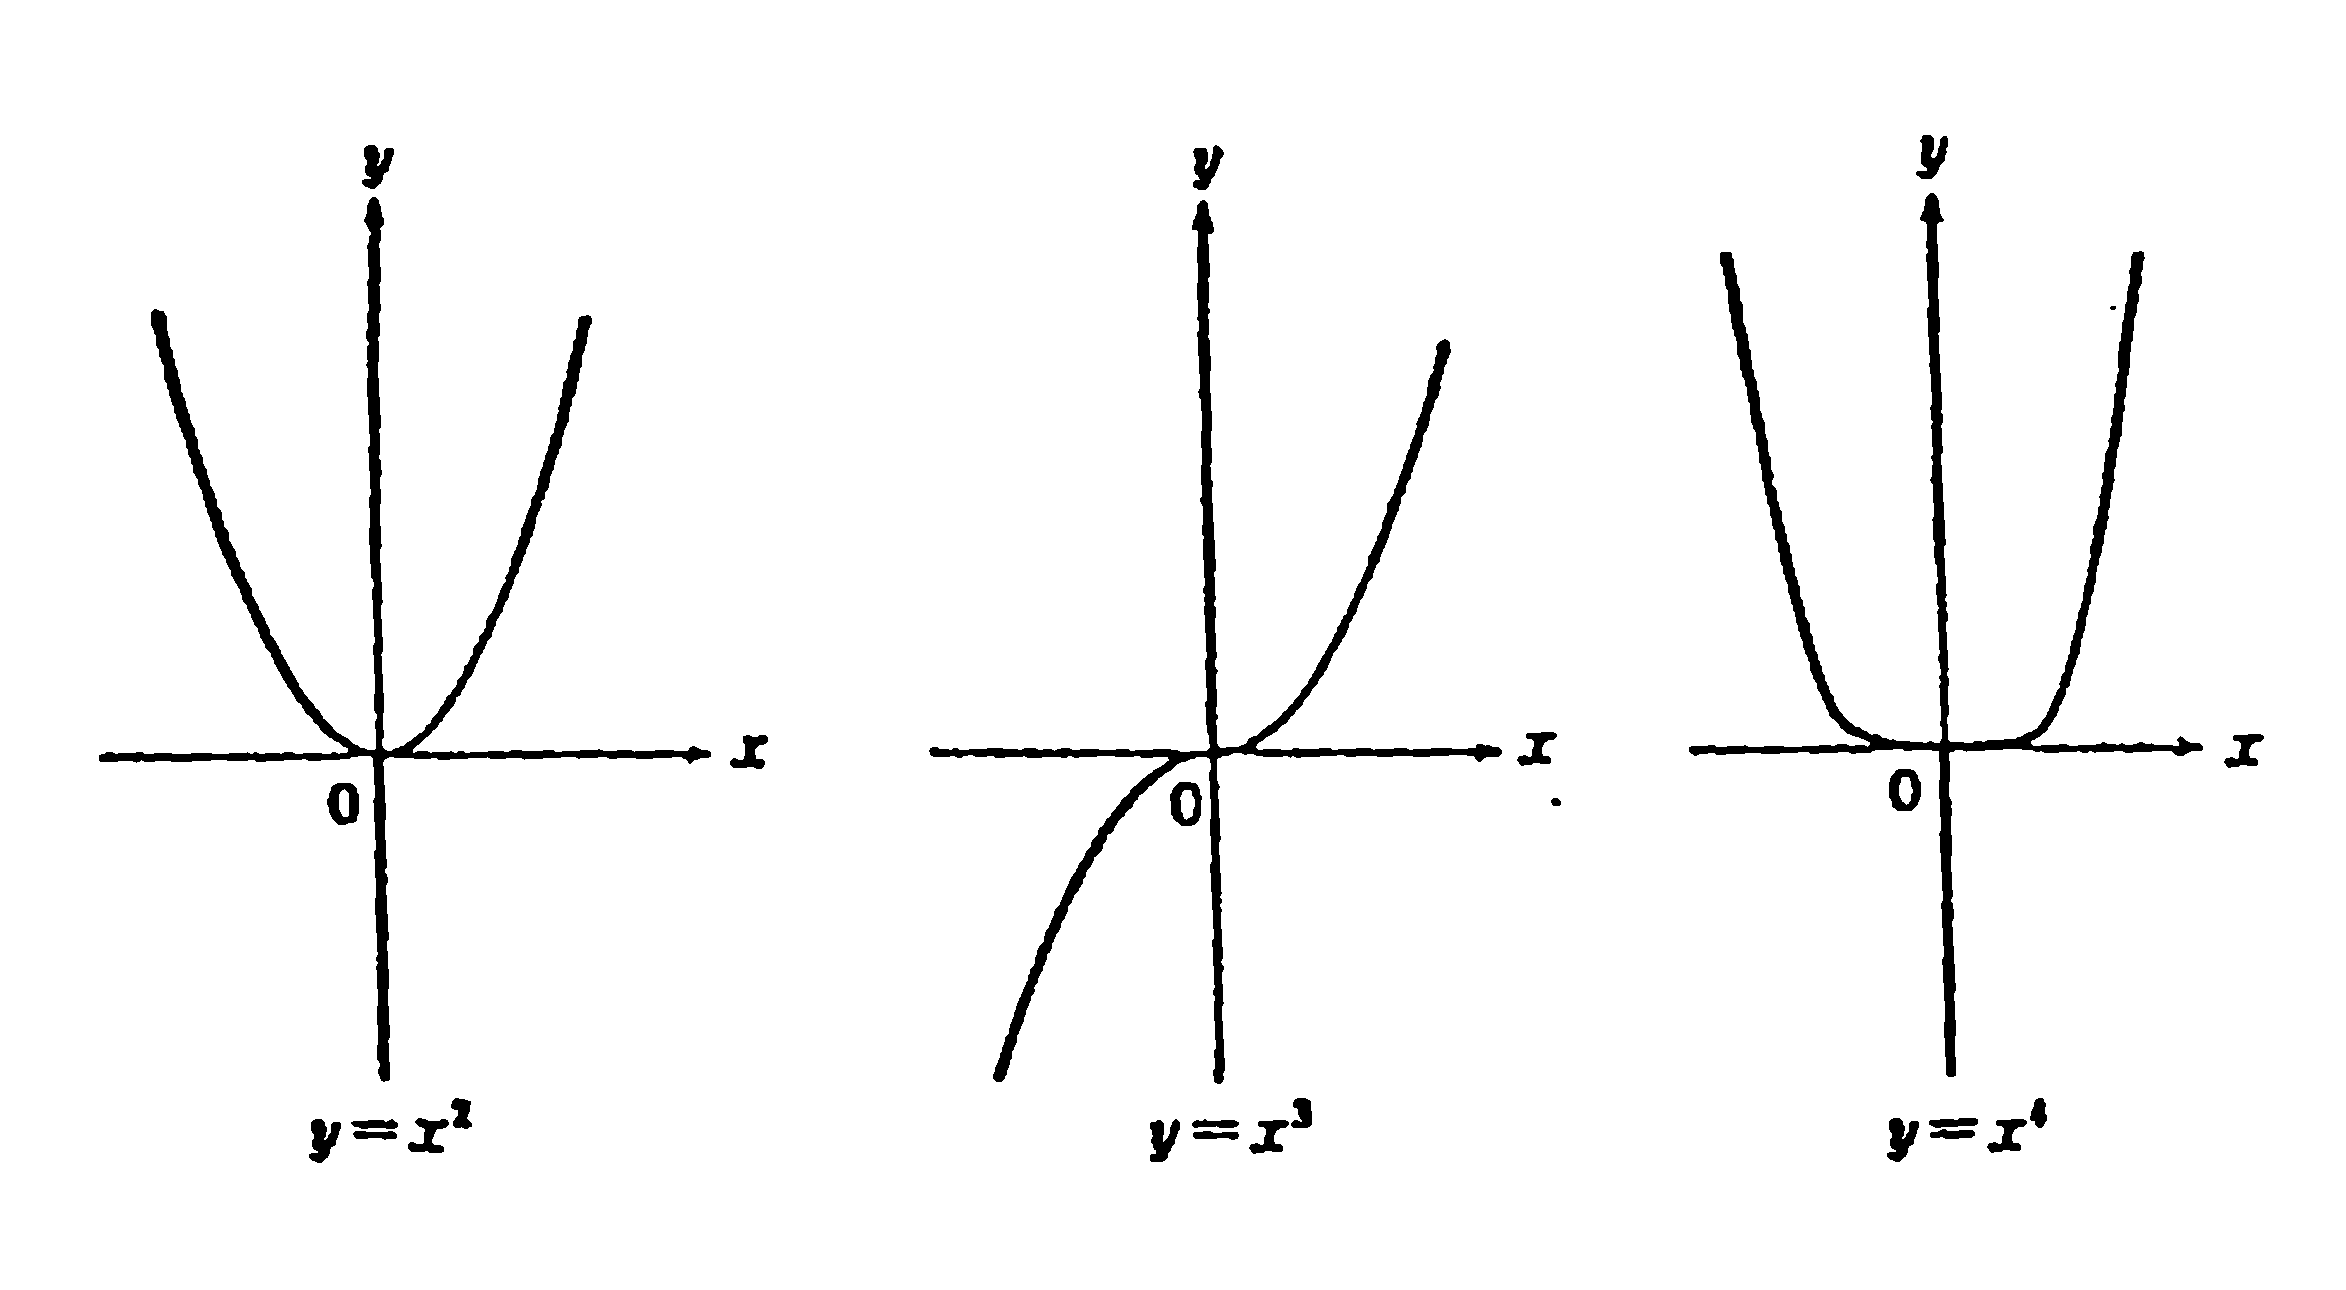
\includegraphics[width=\textwidth]{1-1.png}
    \caption{Графики функций $y = x^2$, $y = x^3$ и $y = x^4$.}
    \label{fig:power_functions}
    \end{figure}
    
    Найдём критические точки возмущённой квадратичной функции:
    \begin{equation}
    y = x^2 + ax + b.
    \label{eq:quad_perturbed}
    \end{equation}
    
    Её производная равна
    \[ y' = 2x + a. \]
    
    Точка $x = -a/2$, в которой производная принимает нулевое значение, является единственной критической точки функции (\ref{eq:quad_perturbed}). Поскольку вторая производная $y'' = 2$, данная критическая точка также будет невырожденной. Нестрого говоря, при <<шевелении>> функции невырожденная критическая точка также <<шевелится>> --- смещается на расстояние $a/2$ --- и остаётся невырожденной; новых критических точек не появляется.
    
    Теперь рассмотрим случай вырожденной критической точки. Производная возмущённой кубической функции
    \begin{equation}
    y = x^3 + ax + b
    \label{eq:cubic_perturbed}
    \end{equation}
    %
    равна
    %
    \[ y' = 3x^2 + a. \]
    %
    и принимает нулевое значение при
    %
    \begin{equation}
    x = \pm\sqrt{-\frac{a}{3}}.
    \label{eq:cubic_solutions}
    \end{equation}
    
    Решения (\ref{eq:cubic_solutions}) являются комплексными при $a > 0$, так что у возмущённой кубической функции при $a > 0$ теряется критическая точка.
    
    Если $a < 0$, то значения $x$ (\ref{eq:cubic_solutions}) вещественны и, следовательно, у функции есть две критические точки. Поскольку вторая производная $y = 6x$ принимает ненулевые значения при $x = \pm\sqrt{-a/3}$, эти критические точки невырождены.
    
    Получаем (см. рисунок \ref{fig:cubic_function}), что вырожденная критическая точка $x = 0$ функции $y = x^3$ при <<шевелении>> исчезает $(a > 0)$, либо разделяется на две невырожденные критические точки $(a < 0)$.
    
    Можно сказать, что в некотором смысле невырожденные точки являются <<устойчивыми>>, а вырожденные --- <<неустойчивыми>> относительно линейного возмущения.
    
    \begin{figure}[ht]
    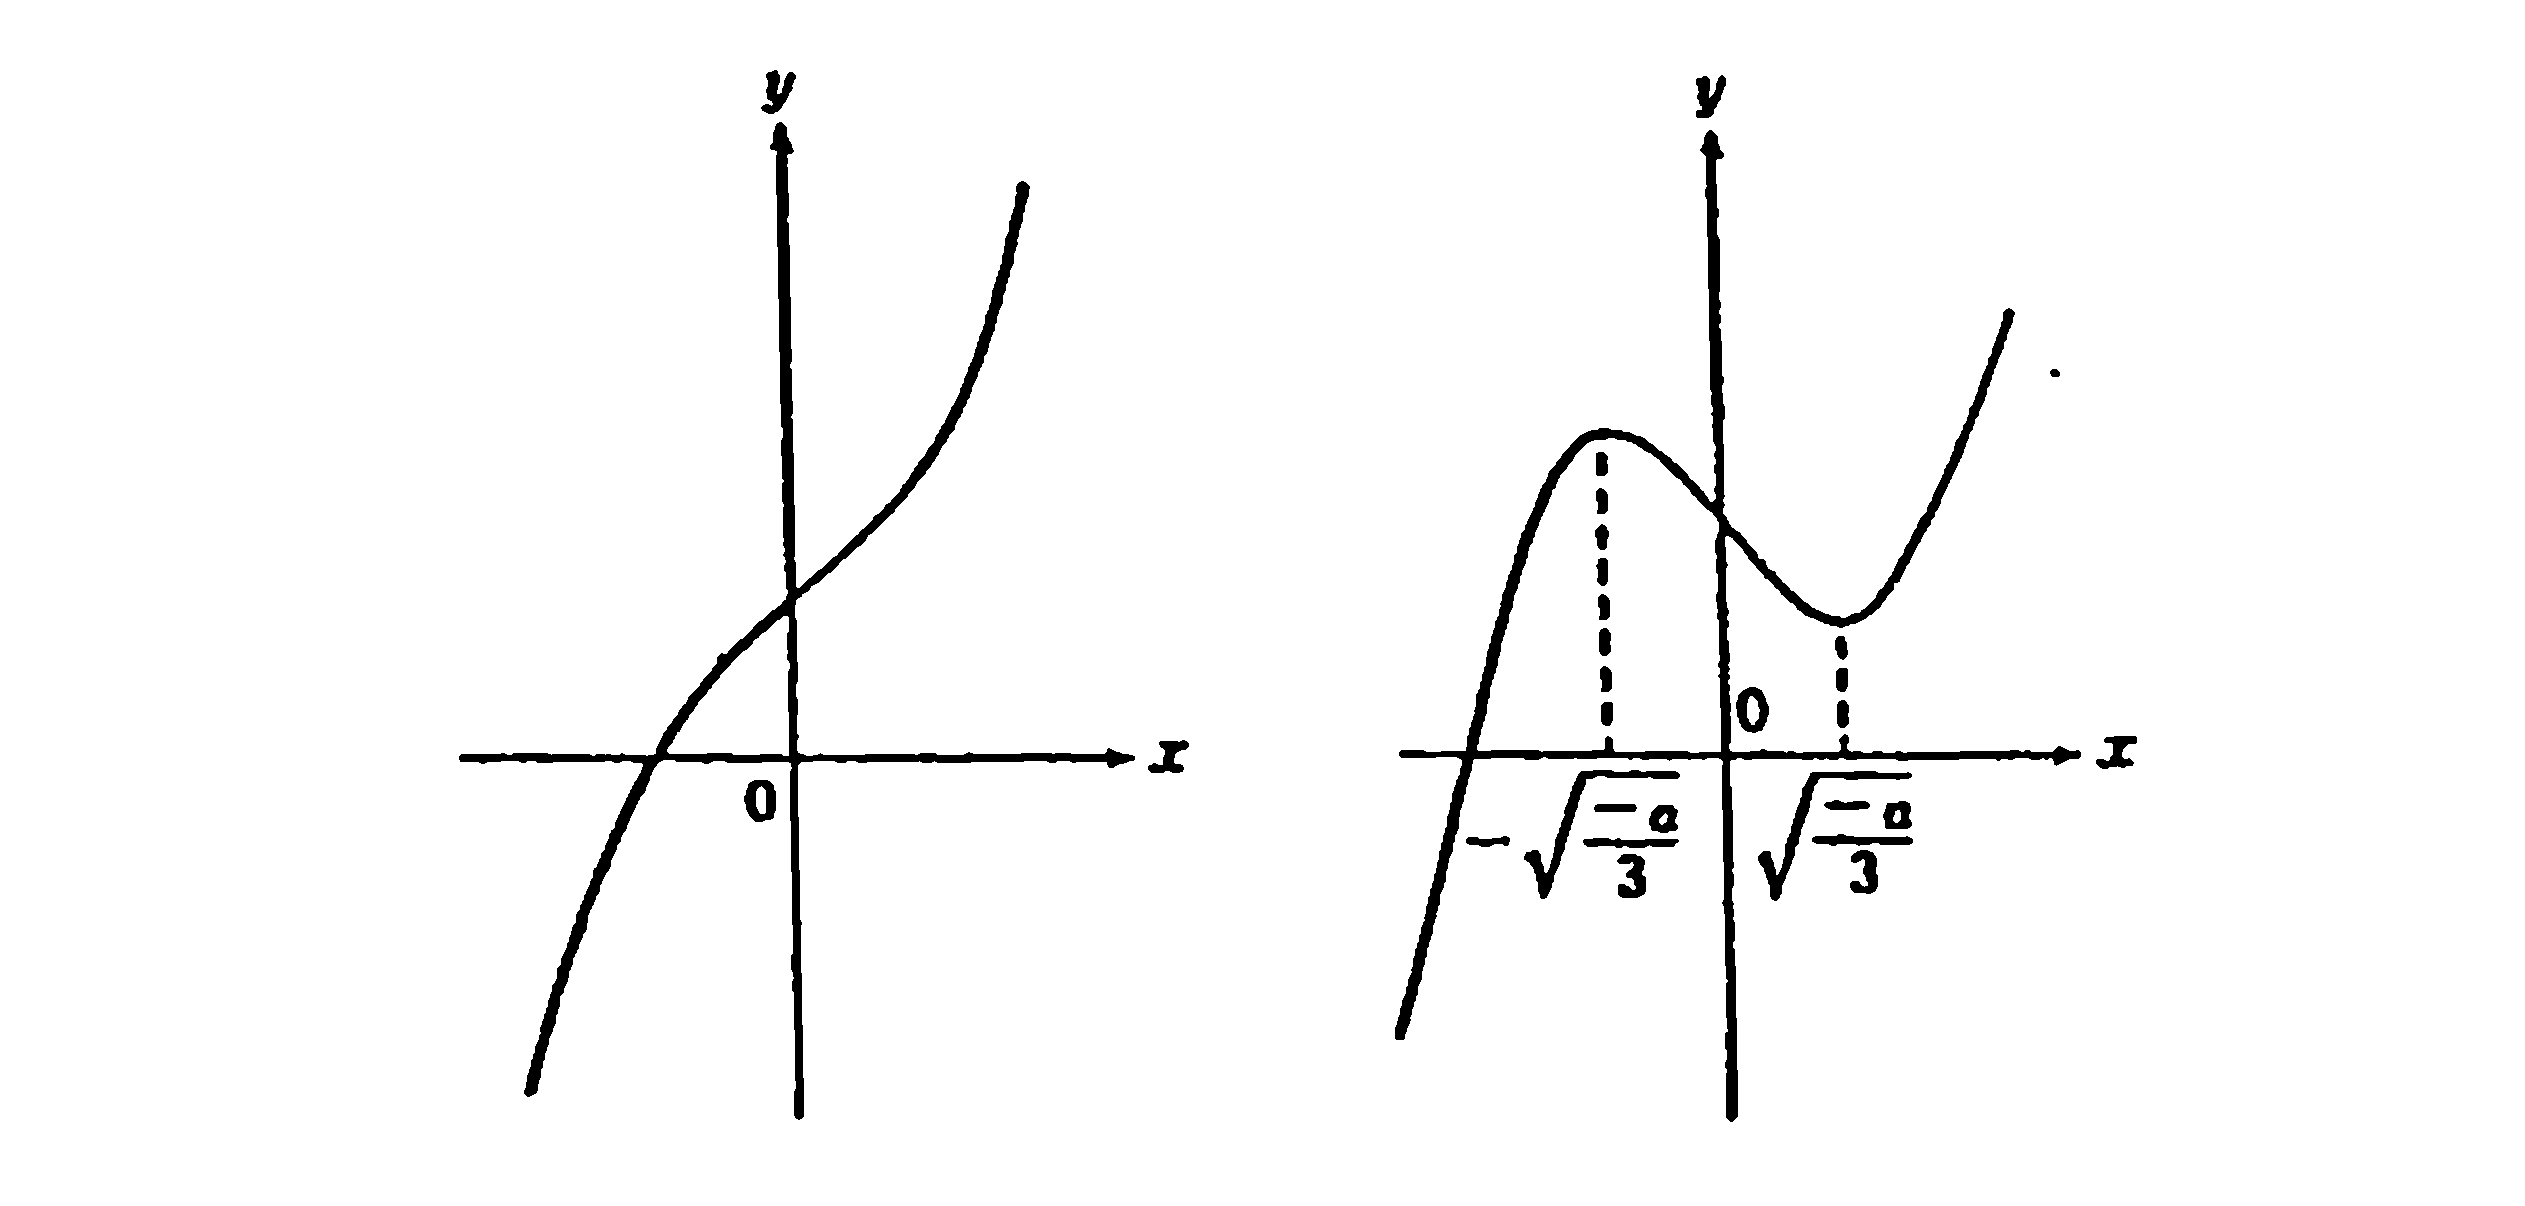
\includegraphics[width=\textwidth]{1-2.png}
    \caption{Графики функции $y = x^3 + ax + b$ при $a > 0$ (слева) и $a < 0$ (справа).}
    \label{fig:cubic_function}
    \end{figure}
    
    \section{Гессиан}
    
    Теперь рассмотрим вещественнозначную функцию
    \begin{equation}
    z = f(x, y)
    \label{eq:z_function}
    \end{equation}
    двух вещественных переменных $x$ и $y$. Будем считать пары аргументов $(x, y)$ точками на плоскости. Тогда $f$ --- функция, каждой точке плоскости сопоставляющая вещественное число, и мы можем изобразить её график в трёхмерном пространстве (см. рисунок \ref{fig:3d_function_graph}).
    
    \begin{figure}[ht]
    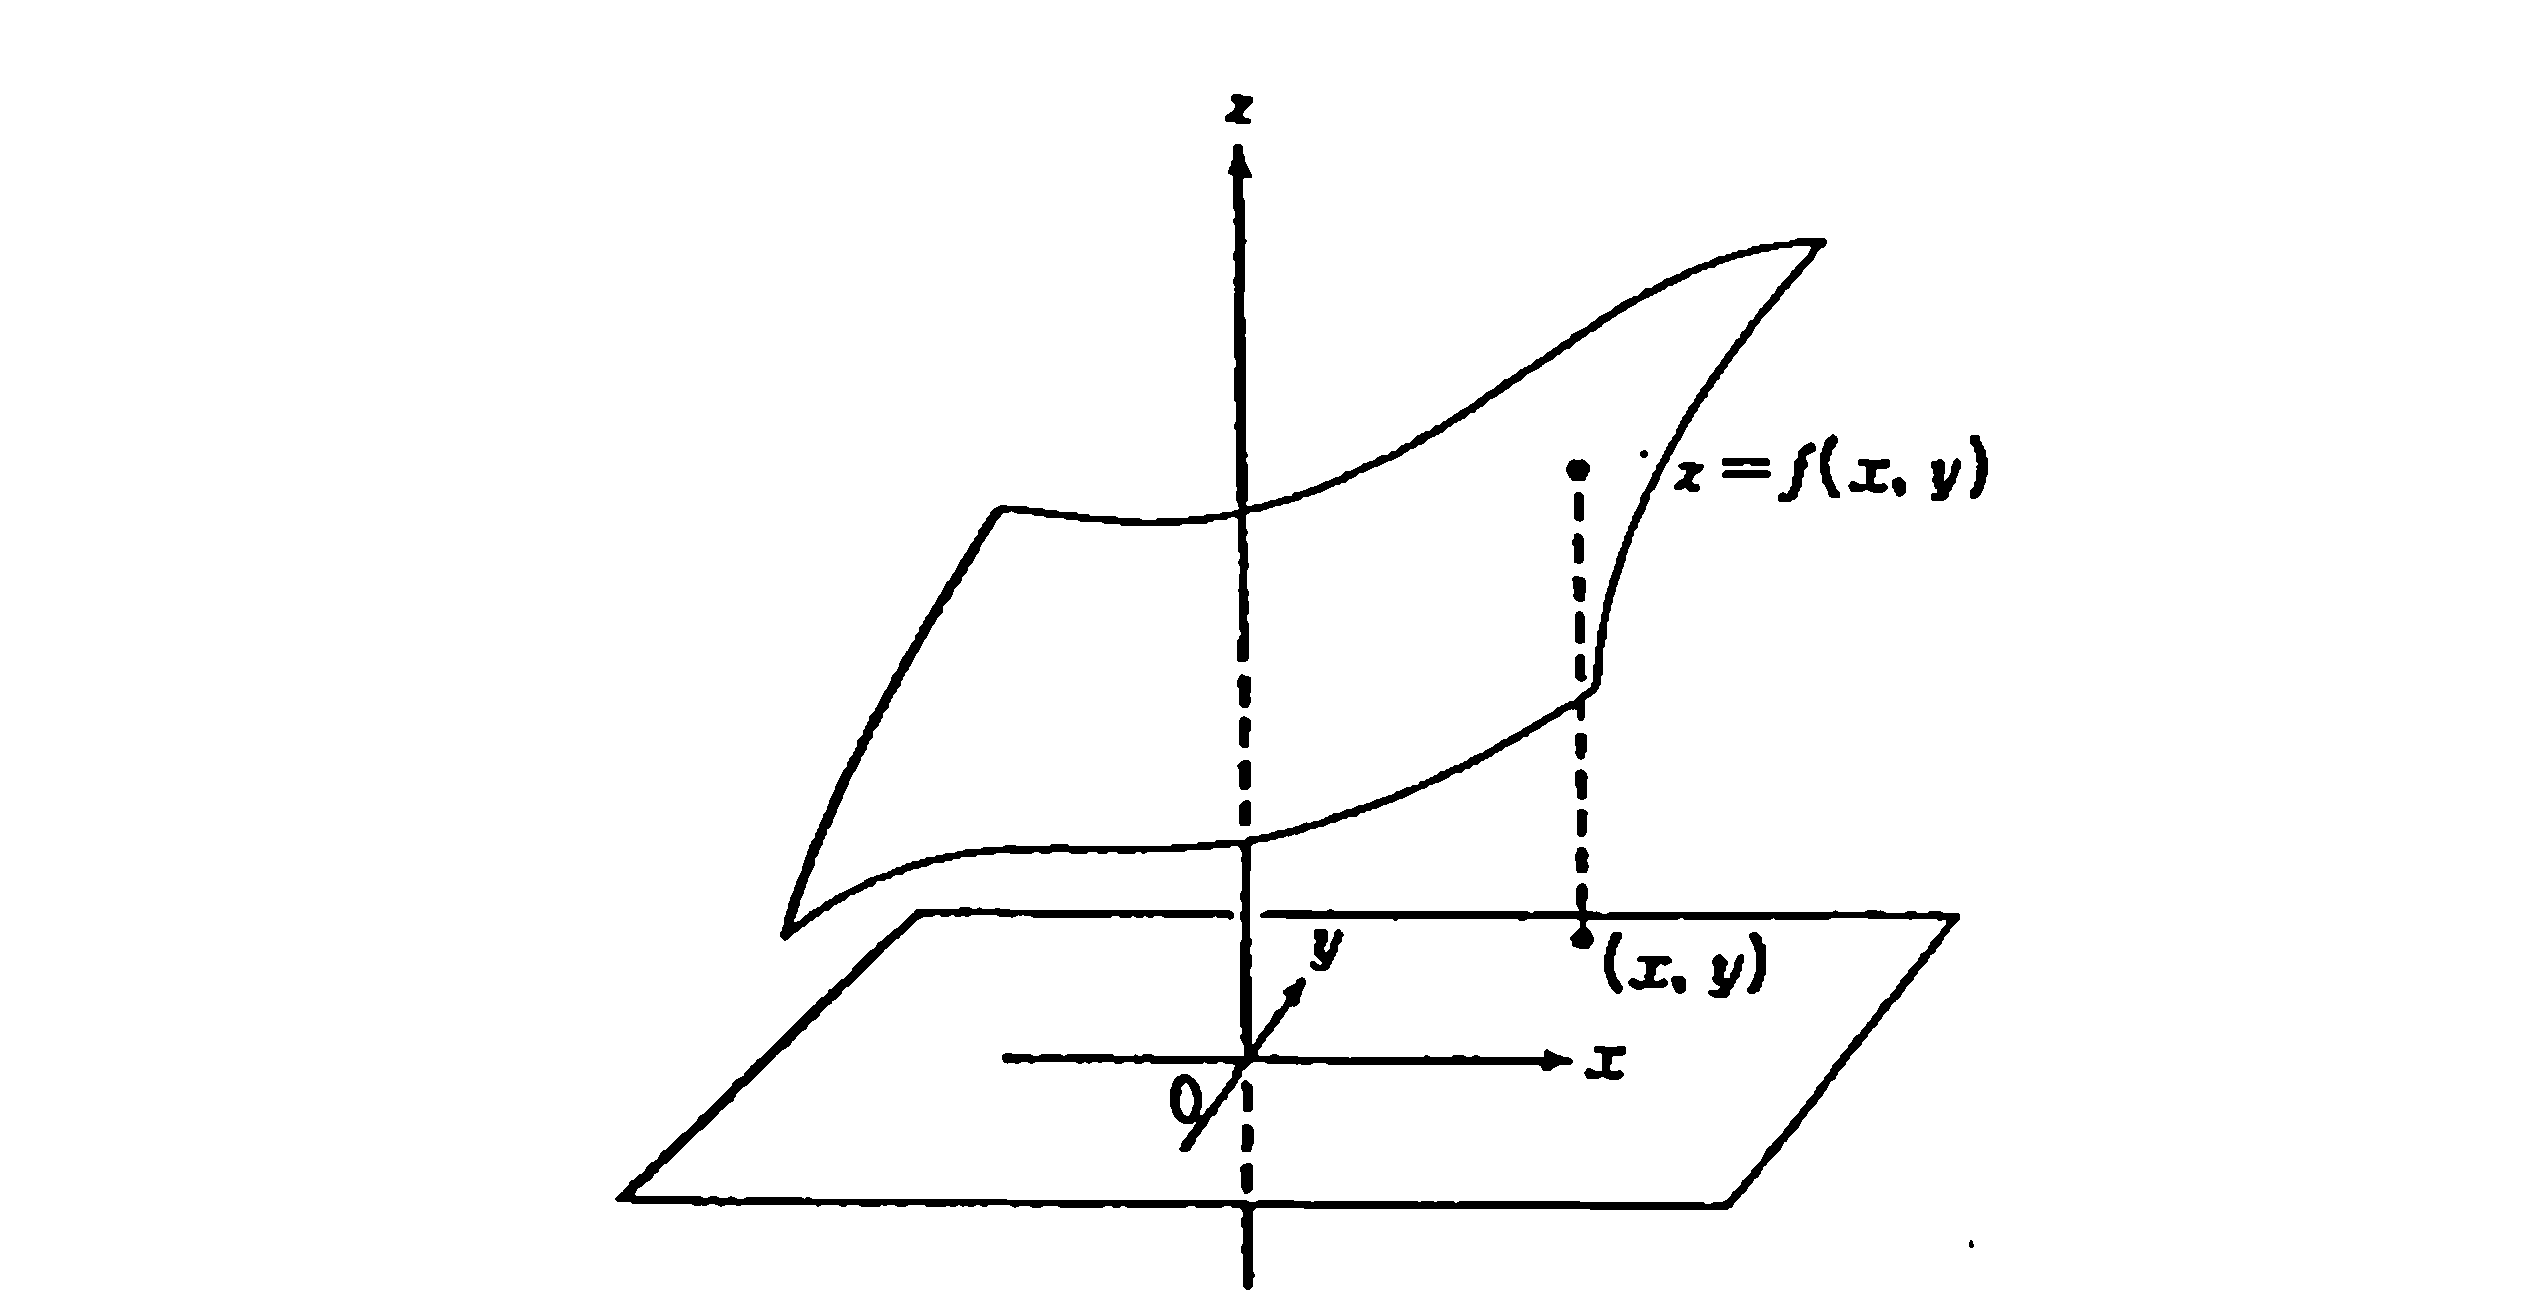
\includegraphics[width=\textwidth]{1-3.png}
    \caption{Пример графика функции двух переменных.}
    \label{fig:3d_function_graph}
    \end{figure}
    
    \begin{definition} (Критические точки функции двух переменных)
    Точка $p_0 = (x_0, y_0)$ называется \emph{критической точкой} функции $z = f(x, y)$, если выполнено условие:
    \begin{equation}
    \frac{\d f}{\d x}(p_0) = 0,\quad \frac{\d f}{\d y}(p_0) = 0.
    \label{eq:crit_point_2d}
    \end{equation}
    \label{def:crit_point_2d}
    \end{definition}
    
    В этом определении мы предполагаем, что $f(x, y)$ принадлежит классу $C^{\infty}$, т.~е. бесконечно дифференцируема. В этой книге мы будем рассматривать только функции класса $C^{\infty}$.
    
    \begin{example}
    Точка $O = (0, 0)$ является критической точкой следующих трёх функций:
    \begin{equation}
    z = x^2 + y^2,\quad z = x^2 - y^2,\quad z = -x^2 - y^2.
    \label{eq:three_functions_2d}
    \end{equation}
    (см. рисунок \ref{fig:three_functions_2d}).
    \label{exam:three_functions_2d}
    \end{example}
    
    \begin{figure}[t]
    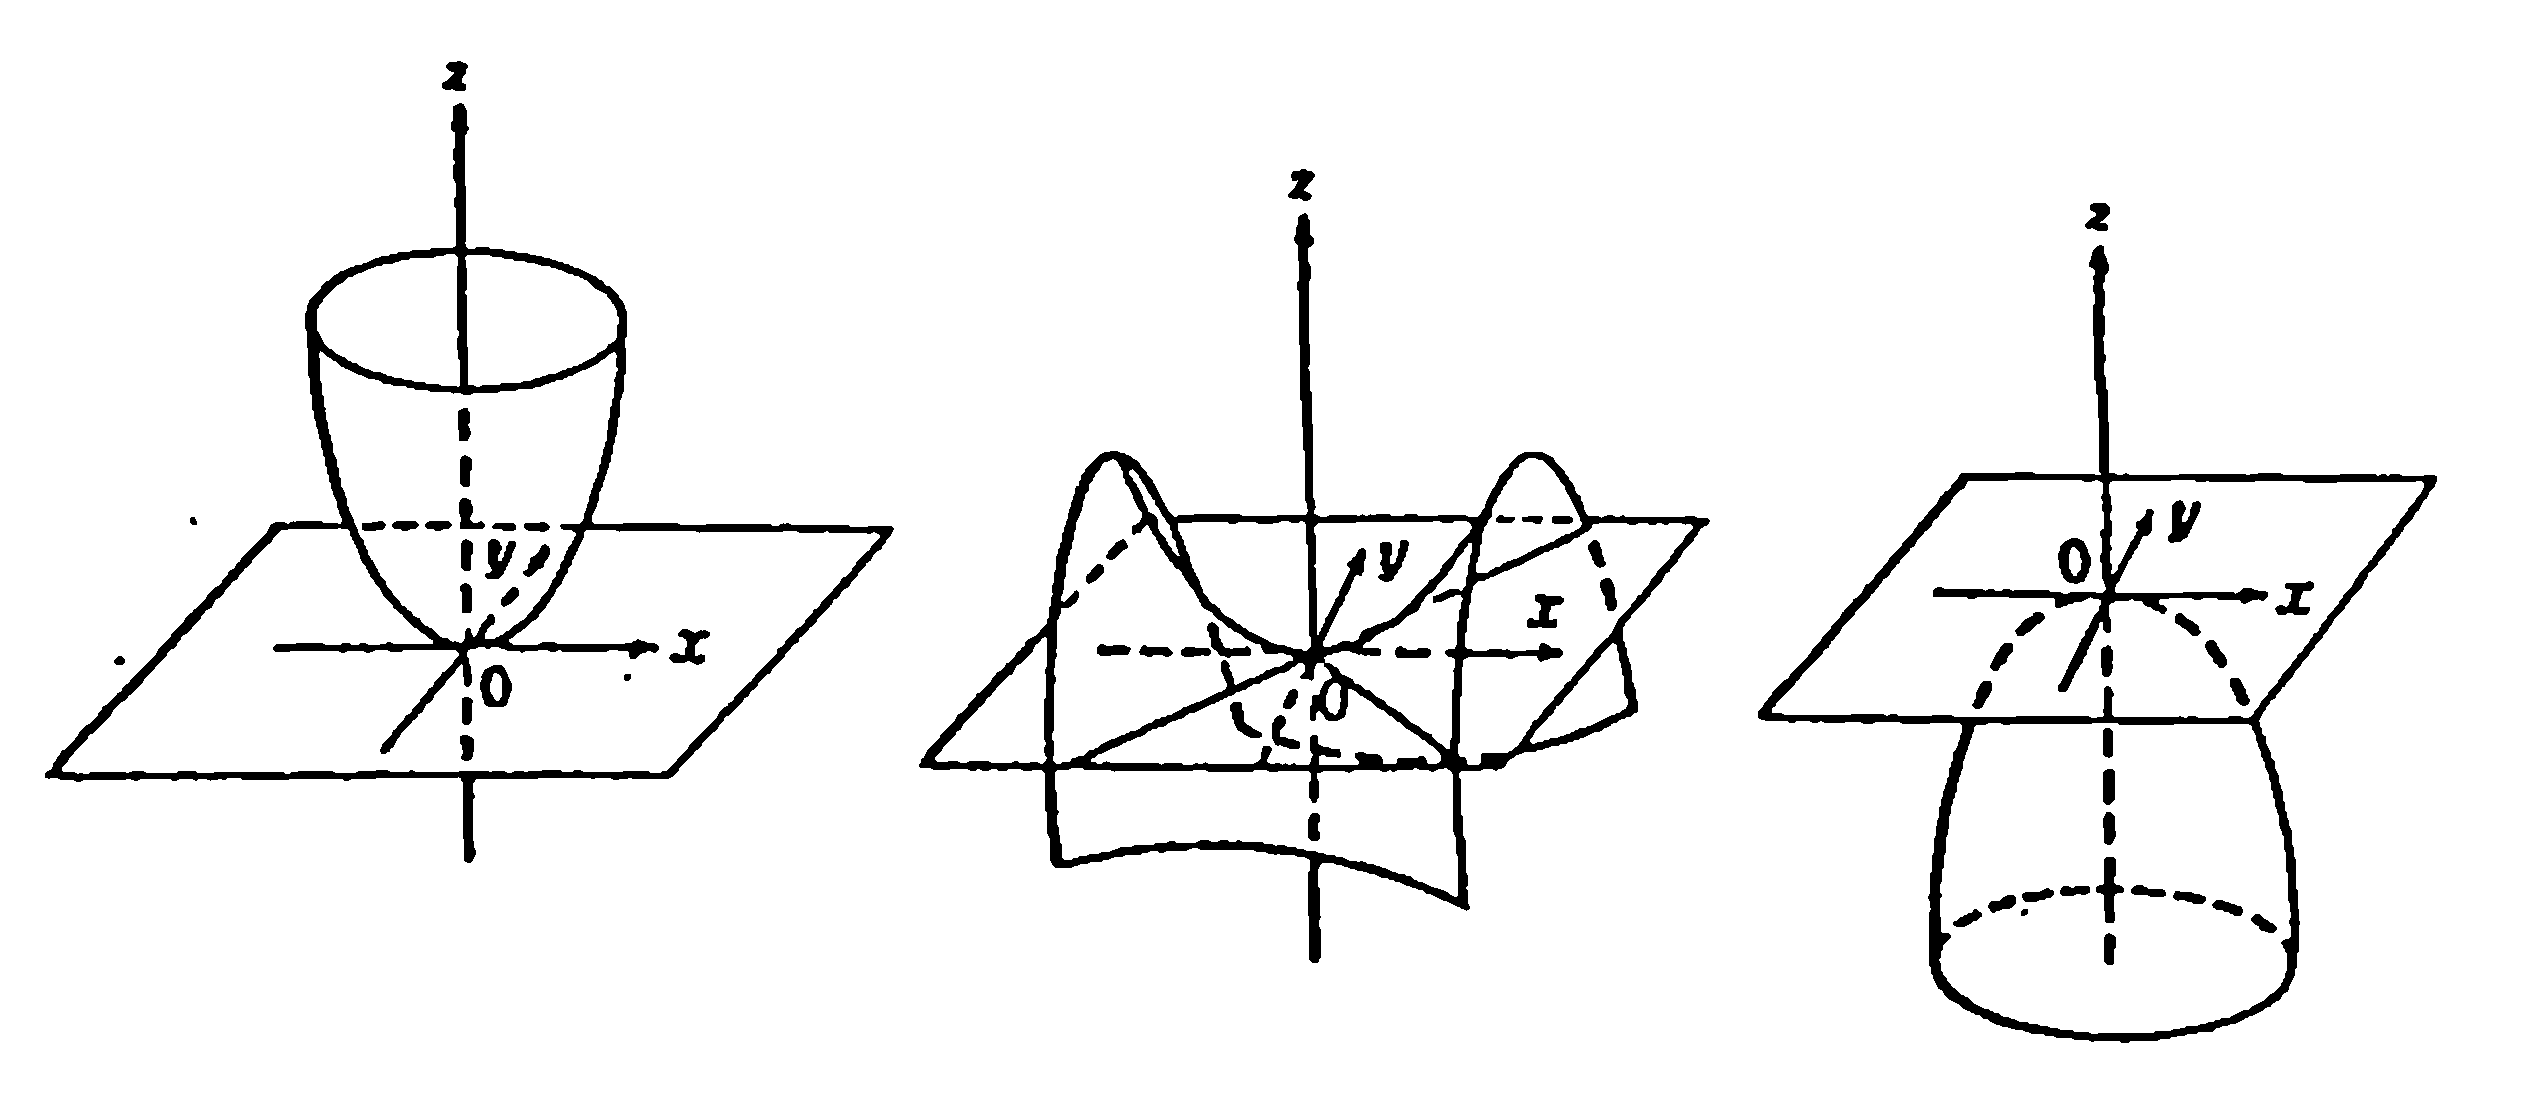
\includegraphics[width=\textwidth]{1-4.png}
    \caption{Слева направо: графики функций $z = x^2 + y^2$, $z = x^2 - y^2$, $z = -x^2 - y^2$.}
    \label{fig:three_functions_2d}
    \end{figure}
    
    Зададимся вопросом: как определить вырожденные и невырожденные критические точки в двумерном случае?
    
    После некоторого раздумья, у читателя может возникнуть искушение сказать, что критическая точка является невырожденной, если
    \begin{equation}
    \frac{\d^2 f}{\d x^2}(p_0) \neq 0,\quad \frac{\d^2 f}{\d y^2}(p_0) \neq 0.
    \label{eq:degenerate_crit_point_2d_wrong}
    \end{equation}
    
    Однако, такое определение плохо тем, что условия (\ref{eq:degenerate_crit_point_2d_wrong}) для той же функции $f$ и точки $p_0$ могут перестать выполняться после замены координат (см. пример \ref{exam:z_xy}). Мы же хотим обобщить понятие невырожденной (и вырожденной) критической точки так, чтобы оно не зависело от выбора системы координат. Следующее определение удовлетворяет этому условию.
    
    \begin{definition} (i)
    Пусть $p_0 = (x_0, y_0)$ --- критическая точка функции $z = f(x, y)$. Матрица
    \begin{equation}
\left(
  \begin{array}{cc}
    \dfrac{\d^2 f}{\d x^2}(p_0) & \dfrac{\d^2 f}{\d x \d y}(p_0)\\
    \dfrac{\d^2 f}{\d y \d x}(p_0) & \dfrac{\d^2 f}{\d y^2}(p_0)
  \end{array}
\right)
    \label{eq:hessian_2d}
    \end{equation}
    вторых производных, вычисленных в точке $p_0$, называется \emph{матрицей Гессе} функции $z = f(x, y)$ в критической точке $p_0$, и обозначается $\mathcal{H}_f(p_0)$. Определитель матрицы Гессе называется \emph{гессианом}.
    
    (ii) Критическая точка $p_0$ функции $z = f(x, y)$ называется \emph{невырожденной}, если гессиан функции $f$ в точке $p_0$ принимает нулевое значение; то есть, $p_0$ --- невырожденная критическая точка, если выполнено условие:
\begin{equation}
\det \mathcal{H}_f(p_0) = \dfrac{\d^2 f}{\d x^2}(p_0) \dfrac{\d^2 f}{\d y^2}(p_0) - \left(\dfrac{\d^2 f}{\d x \d y}(p_0)\right)^2 = 0.
\label{eq:nondegeneracy_2d}
\end{equation}

    В противном случае, если $\det \mathcal{H}_f(p_0) = 0$, точка $p_0$ называется \emph{вырожденной критической точкой}.
    \label{eq:hessian}
    \end{definition}
    
    Заметим, что матрица $\mathcal{H}_f(p_0)$ симметрична, поскольку $\dfrac{\d^2 f}{\d x \d y}(p_0) = \dfrac{\d^2 f}{\d y \d x}(p_0)$.
    
    \begin{example}
    Вычислим матрицу Гессе для функций из примера \ref{exam:three_functions_2d} в точке $(0, 0)$.
    
    (i) Матрица Гессе в нуле функции $z = x^2 + y^2$  равна
    \[
    \left(
  \begin{array}{cc}
    2 & 0\\
    0 & 2
  \end{array}
    \right).
    \]
    
    (ii) Матрица Гессе в нуле функции $z = x^2 - y^2$  равна
    \[
    \left(
  \begin{array}{cc}
    2 & 0\\
    0 & -2
  \end{array}
    \right).
    \]
    
    (iii) Матрица Гессе в нуле функции $z = -x^2 - y^2$  равна
    \[
    \left(
  \begin{array}{cc}
    -2 & 0\\
    0 & -2
  \end{array}
    \right).
    \]
    
    Определители всех перечисленных матриц не равны нулю, поэтому точка $(0, 0)$ будет невырожденной критической точкой всех трёх функций.
    
    \label{exam:three_function_hessians}
    \end{example}
    
    \begin{example}
    Рассмотрим функцию $z = xy$. Точка $(0, 0)$ является критической. Матрица Гессе в нуле равна 
    \[
    \left(
  \begin{array}{cc}
    0 & 1\\
    1 & 0
  \end{array}
    \right),
    \]
    и её определитель не равен нулю, поэтому $(0, 0)$ --- невырожденная критическая точка. Заметим, что функция $z = xy$ получается из функции $z = x^2 - y^2$ заменой координат.
    \label{exam:z_xy}
    \end{example}
    
    \begin{example}
    Точка $(0, 0)$ является критической для функции $z = x^2 + y^3$, однако определитель матрицы Гессе этой функции в нуле
    \[
    \left(
  \begin{array}{cc}
    2 & 0\\
    0 & 0
  \end{array}
    \right)
    \]
    равен нулю. Следовательно, (0, 0) --- вырожденная критическая точка функции $z = x^2 + y^3$.
    \end{example}
    
    Как изменяется матрица Гессе при замене координат?
    
    \begin{lemma}
    Пусть $p_0$ --- критическая точка функции $z = f(x, y)$. Обозначим за $\mathcal{H}_f(p_0)$ матрицу Гессе, вычисленную в координатах $(x, y)$, и за $\widetilde{\mathcal{H}}_f(p_0)$ матрицу Гессе, вычисленную в других координатах $(X, Y)$. Тогда верно соотношение:
    \begin{equation}
    \widetilde{\mathcal{H}}_f(p_0) = J^T(p_0)\mathcal{H}_f(p_0)J(p_0),
    \end{equation}
    где $J(p_0)$ --- матрица Якоби замены координат, определённая как
    \begin{equation}
    \left(
  \begin{array}{cc}
    \dfrac{\d x}{\d X}(p_0) & \dfrac{\d x}{\d Y}(p_0)\\
    \dfrac{\d y}{\d X}(p_0) & \dfrac{\d y}{\d Y}(p_0)
  \end{array}
    \right),
    \end{equation}
    и $J^T(p_0)$ --- транспонированная матрица Якоби.
    \label{lm:hessian_transform_2d}
    \end{lemma}
    
    \begin{proof}
    Доказательство предлагается провести читателю самостоятельно. Идея заключается в замене
\[
  \begin{array}{cc}
    \dfrac{\d f}{\d X} = \dfrac{\d f}{\d x}\dfrac{\d x}{\d X} + \dfrac{\d f}{\d y}\dfrac{\d y}{\d X},\\
    \dfrac{\d f}{\d Y} = \dfrac{\d f}{\d x}\dfrac{\d x}{\d Y} + \dfrac{\d f}{\d y}\dfrac{\d y}{\d Y}
  \end{array}
\]
  и последующем выражении $\dfrac{\d^2 f}{\d X^2}$, $\dfrac{\d^2 f}{\d X \d Y}$ и $\dfrac{\d^2 f}{\d Y^2}$ через $\dfrac{\d^2 f}{\d x^2}$, $\dfrac{\d^2 f}{\d x \d y}$ и $\dfrac{\d^2 f}{\d y^2}$. Затем нужно вычислить эти производные в точке $p_0$, не забывая, что $\dfrac{\d f}{\d x}(p_0) = \dfrac{\d f}{\d y}(p_0) = 0$, и сравнить результат с произведением матриц из правой части.
    \end{proof}
    
    \begin{example}
    Перепишем функцию $z = xy$ (Пример \ref{exam:z_xy}) в новых координатах
    \begin{equation}
    \begin{cases}
    x = X + Y,\\
    y = X - Y.
    \end{cases}
    \label{eq:coord_transform}
    \end{equation}
    
    Получим
    \[
    xy = (X - Y)(X + Y) = X^2 - Y^2,
    \]
    
    т.~е. вторую функцию из Примера \ref{exam:three_functions_2d}. Матрицы Гессе в нуле относительно координат $(x, y)$ и $(X, Y)$ равны, соответсвенно,
    \[
\left(
  \begin{array}{cc}
    0 & 1\\
    1 & 0
  \end{array}
\right),
    \quad
\left(
  \begin{array}{cc}
    2 & 0\\
    0 & -2
  \end{array}
\right).
    \]
    
    Матрица Якоби преобразования координат (\ref{eq:coord_transform}) равна
    \[
\left(
  \begin{array}{cc}
    1 & -1\\
    1 & 1
  \end{array}
\right).
    \]
    
    Убедимся, что утверждение Леммы \ref{lm:hessian_transform_2d} выполняется:
    \[
\left(
  \begin{array}{cc}
    2 & 0\\
    0 & -2
  \end{array}
\right) = 
\left(
  \begin{array}{cc}
    1 & 1\\
    -1 & 1
  \end{array}
\right)
\left(
  \begin{array}{cc}
    0 & 1\\
    1 & 0
  \end{array}
\right)
\left(
  \begin{array}{cc}
    1 & -1\\
    1 & 1
  \end{array}
\right).
\]
    \end{example}
    
\begin{corollary} (из Леммы \ref{lm:hessian_transform_2d}) Свойства невырожденности и вырожденности критической точки не зависят от выбора координат.
\label{corol:degeneracy_2d}
\end{corollary}

\begin{proof}
Перейдём к определителям в равенстве из утверждения $\widetilde{\mathcal{H}}_f(p_0) = J^T(p_0)\mathcal{H}_f(p_0)J(p_0)$ Леммы \ref{lm:hessian_transform_2d}: 

\begin{equation}
\det\widetilde{\mathcal{H}}_f(p_0) = \det J^T(p_0)\det\mathcal{H}_f(p_0)\det J(p_0).
\end{equation}

Заметим, что якобиан преобразования координат
\begin{equation}
\det J(p_0) \neq 0,
\end{equation}
поэтому $\det\widetilde{\mathcal{H}}_f(p_0) = 0$ тогда и только тогда, когда $\det\mathcal{H}_f(p_0) = 0$, откуда следует утверждение Cледствия \ref{corol:degeneracy_2d}.    
\end{proof}

\section{Лемма Морса}
В этом разделе мы докажем следующий факт.

\begin{theorem} (Лемма Морса). Пусть $p_0$ --- невырожденная критическая точка функции $f$ двух переменных. Тогда существуют локальные координаты $(X, Y)$, в которых функция $f$ принимает одну из трёх стандартных форм:
%
\[
  \begin{array}{rl}
   (i) & f = X^2 + Y^2 + c,\\
   (ii) & f = X^2 - Y^2 + c,\\
   (iii) & f = -X^2 - Y^2 + c,
  \end{array}
\]
%
где $c = f(p_0)$, а $p_0$ --- нуль новой системы координат ($p_0 = (0, 0)$).
\label{thm:morse_lemma_2d}
\end{theorem}

Эта теорема утверждает, что функция в окрестности невырожденной критической точки ведёт себя предельно просто: подходящая замена координат приводит в случаю одной из трёх простых функций, рассмотренных в Примере \ref{exam:three_functions_2d}.

Поскольку ни у одной из этих функций нет критических точек, близких к нулю, верно следующее утверждение.

\begin{corollary}
Невырожденные критические точки функции двух переменных изолированы.
\label{corol:crit_points_isolated_2d}
\end{corollary}

Это утверждение верно и в общем случае, для функции $m$ переменных.

Теперь докажем Теорему \ref{thm:morse_lemma_2d}.

\begin{proof}
Рассмотрим произвольную систему координат в окрестности точки $p_0$. Пусть $p_0$ --- точка $(0, 0)$ в этих координатах. Также для простоты изложения будем считать\footnote{В общем случае можно рассмотреть функцию $g(x) = f(x) - f(p_0)$ и применить к ней все дальнейшие рассуждения}, что $f(p_0) = 0$. Далее мы покажем, что, не ограничивая общности, мы можем положить
\begin{equation}
\dfrac{\d^2 f}{\d x^2}(p_0) \neq 0.
\label{eq:second_derivative_condition_2d}
\end{equation}
Если в нашей системе координат $\dfrac{\d^2 f}{\d x^2}(p_0) \neq 0$, то доказывать нечего. Если $\dfrac{\d^2 f}{\d x^2}(p_0) = 0$, но $\dfrac{\d^2 f}{\d y^2}(p_0) \neq 0$, то мы можем просто поменять местами оси $x$ и $y$, чтобы условие (\ref{eq:second_derivative_condition_2d}) выполнялось. Рассмотрим случай, когда $\dfrac{\d^2 f}{\d x^2}(p_0) = 0$ и $\dfrac{\d^2 f}{\d y^2}(p_0) = 0$.

В этом случае матрица Гессе в точке $p_0 = (0, 0)$ выглядит так:

\begin{equation}
\left(
  \begin{array}{rl}
   0 & a\\
   a & 0
  \end{array}
\right).
\end{equation}

Поскольку $p_0$ --- невырожденная критическая точка, $a \neq 0$. Введём новые локальные координаты $(X, Y)$:

\begin{equation}
x = X + Y,\quad y = X - Y.
\end{equation}

Матрица Якоби перехода от координат $(X, Y)$ к $(x, y)$:

\begin{equation}
J =
\left(
  \begin{array}{cc}
   1 & -1\\
   1 & 1
  \end{array}
\right).
\end{equation}

Пользуясь Леммой \ref{lm:hessian_transform_2d}, вычислим матрицу Гессе $\widetilde{\mathcal{H}}_f$ в координатах $(X, Y)$:

\begin{equation}
\widetilde{\mathcal{H}}_f = J^T \mathcal{H}_f J =
\left(
  \begin{array}{cc}
   2a & 0\\
   0 & -2a
  \end{array}
\right).
\end{equation}

Мы видим, что в новых координатах

\begin{equation}
\dfrac{\d^2 f}{\d X^2}(p_0) = 2a \neq 0,\quad \dfrac{\d^2 f}{\d Y^2}(p_0) = -2a \neq 0.
\end{equation}

Для удобства будем обозначать новые координаты $(X, Y)$ как $(x, y)$. Заметим, что теперь условие 
\ref{eq:second_derivative_condition_2d} выполнено, и мы можем продолжить доказательство в предположении \ref{eq:second_derivative_condition_2d}.

В анализе функций многих переменных известен следующий факт. Пусть функция $z = f(x, y)$ задана в окрестности нуля и $f(0, 0) = 0$. Тогда существуют функции $g(x, y)$ и $h(x, y)$ такие, что
\begin{equation}
f(x, y) = x g(x, y) + y h(x, y)
\label{eq:func_decomposition_2d}
\end{equation}
в некоторой окрестности нуля, и 
\begin{equation}
\dfrac{\d f}{\d x}(0, 0) = g(0, 0),\quad \dfrac{\d f}{\d y}(0, 0) = h(0, 0).
\label{eq:func_decomposition_2d_zero_condition}
\end{equation}
Этот факт достаточно известен, но для удобства читателя мы его докажем ниже.

Для простоты скажем, что $z = f(x, y)$ определена на всей плоскости $Oxy$. Фиксируем произвольную точку $(x, y)$. Рассмотрим функцию $f(xt, yt)$ с параметром $t$. Если мы продифференцируем эту функцию по параметру $t$, а затем проинтегрируем, мы получим исходную функцию. В частности, рассмотрим определённый интеграл от $0$ до $1$ и воспользуемся условием $f(0, 0) = 0$:
\begin{multline}
f(x, y) = \int_0^1 \dfrac{df(tx, ty)}{dt} dt = \int_0^1 \left\{x\dfrac{df}{dx}(tx, ty) + y\dfrac{df}{dy}(tx, ty)\right\} dt =\\= x g(x, y) + y h(x, y).
\end{multline}

% В следующем абзаце пояснения, как для детей. Я не буду его переводить.

Здесь мы ввели обозначения
\begin{equation}
g(x, y) = \int_0^1 \dfrac{df}{dx}(tx, ty)\,dt,\quad h(x, y) = \int_0^1 \dfrac{df}{dy}(tx, ty)\,dt.
\label{eq:morse_lemma_fg_2d}
\end{equation}

Таким образом, мы нашли функции $g$ и $h$, удовлетворяющие равенству (\ref{eq:func_decomposition_2d}). Более того, подстановкой $(x, y) = (0, 0)$ в (\ref{eq:morse_lemma_fg_2d}) убеждаемся, что равенства (\ref{eq:func_decomposition_2d_zero_condition}) также верны.

Вернёмся к доказательству теоремы. Поскольку $p_0 = (0, 0)$ --- критическая точка функции $f$, мы имеем:

\begin{equation}
g(0, 0) = \dfrac{\d f}{\d x}(0, 0) = 0,\quad h(0, 0) = \dfrac{\d f}{\d y}(0, 0) = 0.
\end{equation}

Теперь применим доказанное выше утверждение к функциям $g(x, y)$ и $h(x, y)$. Существуют функции $h_{11}, h_{12}, h_{21}$ и $h_{22}$, для которых верны соотношения:

\begin{equation}
g(x, y) = x h_{11}(x, y) + y h_{12}(x, y)
\label{eq:func_decomposition_2d_a}
\end{equation}
и
\begin{equation}
h(x, y) = x h_{21}(x, y) + y h_{22}(x, y).
\label{eq:func_decomposition_2d_b}
\end{equation}
Подставим равенства (\ref{eq:func_decomposition_2d_a}) и (\ref{eq:func_decomposition_2d_b}) в (\ref{eq:func_decomposition_2d}):
\begin{equation}
f(x, y) = x^2 h_{11} + xy(h_{12} + h_{21}) + y^2 h_{22}.
\label{eq:morse_lemma_h_functions_2d}
\end{equation}
Введём новые обозначения: $H_{11} = h_{11}$, $H_{12} = (h_{12} + h_{21}) / 2$, $H_{22} = h_{22}$. Приведём (\ref{eq:morse_lemma_h_functions_2d}) к более простому виду:
\begin{equation}
f(x, y) = x^2 H_{11} + xy H_{12} + y^2 H_{22}.
\label{eq:morse_lemma_H_functions_2d}
\end{equation}
Отсюда простыми вычислениями получаем:
\begin{equation}
\begin{cases}
\dfrac{\d^2 f}{\d x^2}(0, 0) = 2H_{11}(0, 0),\\
\dfrac{\d^2 f}{\d x \d y}(0, 0) = \dfrac{\d^2 f}{\d y \d x}(0, 0) = 2H_{12}(0, 0),\\
\dfrac{\d^2 f}{\d y^2}(0, 0) = 2H_{22}(0, 0).
\end{cases}
\label{eq:morse_lemma_H_second_derivatives_2d}
\end{equation}
Теперь вспомним, что левая часть верхнего уравнения не равна нулю. Значит, $H_{11}(0, 0) \neq 0$, а из непрерывности $H_{11}$ следует, что
\begin{equation}
H_{11}(x, y) \neq 0 \text{ в некоторой окрестности точки } (0, 0).
\end{equation}
Введём новую координату $X$ в окрестности нуля:
\begin{equation}
X = \sqrt{|H_{11}|}\left(x + \dfrac{H_{12}}{H_{11}}y\right).
\end{equation} 
Координату $y$ оставим прежней. Поскольку якобиан перехода от $(x, y)$ к $(X, y)$ в точке $(0, 0)$ ненулевой, локальные координаты $(X, y)$ корректно определены в некоторой окрестности нуля. Возведём $X$ в квадрат:
\begin{align}
\begin{split}
X^2 = |H_{11}|\left(x^2 + 2\dfrac{H_{12}}{H_{11}} xy + \dfrac{H^2_{12}}{H^2_{11}} y^2 \right) \\=
\begin{cases}
H_{11}x^2 + 2 H_{12} xy + \dfrac{H^2_{12}}{H_{11}} y^2 & (H_{11} > 0),\\
-H_{11}x^2 - 2 H_{12} xy - \dfrac{H^2_{12}}{H_{11}} y^2 & (H_{11} < 0).
\end{cases}
\end{split}
\label{eq:morse_lemma_x_squared_2d}
\end{align}
Сравнивая (\ref{eq:morse_lemma_x_squared_2d}) и (\ref{eq:morse_lemma_H_functions_2d}), получаем, что при $H_{11} > 0$
\begin{equation}
f = X^2 + \left(H_{22} - \dfrac{H^2_{12}}{H_{11}}\right) y^2,
\label{eq:morse_2d_st_form_a}
\end{equation}
а при $H_{11} < 0$
\begin{equation}
f = -X^2 + \left(H_{22} - \dfrac{H^2_{12}}{H_{11}}\right) y^2.
\label{eq:morse_2d_st_form_b}
\end{equation}

Из равенств (\ref{eq:morse_lemma_H_second_derivatives_2d}) следует, что
\begin{equation}
H_{11}(0, 0) H_{22}(0, 0) - H_{12}^2(0, 0) = \dfrac{1}{4} \det \mathcal{H}_f \neq 0,
\end{equation}
где $\mathcal{H}_f \neq 0$ из условия невырожденности критической точки $p_0$. Теперь выберем новую координату $Y$ в окрестности точки $p_0 = (0, 0)$:
\begin{equation}
Y = \sqrt{\left|\dfrac{H_{11} H_{22} - H_{12}^2}{H_{11}}\right|}y,
\end{equation}
и перепишем равенства (\ref{eq:morse_2d_st_form_a}) и (\ref{eq:morse_2d_st_form_b}). Тогда $f$ представляется в локальных координатах $(X, Y)$ одним из следующих способов:

\begin{equation}
f =
\begin{cases}
X^2 + Y^2 & (H_{11} > 0, K > 0),\\
X^2 - Y^2 & (H_{11} > 0, K < 0),\\
-X^2 + Y^2 & (H_{11} < 0, K < 0),\\
-X^2 - Y^2 & (H_{11} < 0, K > 0),
\end{cases}
\end{equation}
где для краткости мы обозначили $K = H_{11} H_{22} - H_{12}^2$. Если мы поменяем координаты $X$ и $Y$ поворотом на $90^{\circ}$, то заметим, что $f = X^2 - Y^2$ и $f = -X^2 + Y^2$ --- это одна и та же стандартная форма. Это замечание завершает доказательство Теоремы \ref{thm:morse_lemma_2d}.
\end{proof}

\begin{definition} (Индекс невырожденной критической точки). Пусть $p_0$ --- невырожденная критическая точка функции $f$ двух переменных. В подходящей системе координат $(x, y)$ в некоторой окрестности точки $p_0$ функция $f$ представляется в одной из стандартных форм, перечисленных в Теореме \ref{thm:morse_lemma_2d}. \emph{Индексом} невырожденной критической точки $p_0$ назовём число $0$, $1$ или $2$, если функция $f$ принимает вид $f = x^2 + y^2 + c$, $f = x^2 - y^2 + c$ или $f = -x^2 - y^2 + c$, соответственно. Иначе говоря, индекс точки $p_0$ равен количеству знаков <<минус>> в стандартной форме.
\end{definition}
    
Как можно заметить по соответствующим графикам (см. рисунок \ref{fig:three_functions_2d}) функций $f = x^2 + y^2$, $f = x^2 - y^2$ и $f = -x^2 - y^2$, если у точки $p_0$ индекс $0$, то $p_0$ --- точка минимума. Если у $p_0$ индекс $1$, то у функции в любой окрестности точки $p_0$ будут как значения, большие $f(p_0)$, так и значения, меньшие $f(p_0)$. Если у $p_0$ индекс $2$, то $p_0$ --- точка максимума. Таким образом, индекс критической точки $p_0$ определяется поведением функции вблизи $p_0$.

Докажем, что индекс критической точки определён корректно. В Примере \ref{exam:three_function_hessians} мы вычислили матрицы Гессе функций $f = x^2 + y^2$, $f = x^2 - y^2$ и $f = -x^2 - y^2$: они равны
    \[
    \left(
  \begin{array}{cc}
    2 & 0\\
    0 & 2
  \end{array}
    \right),\;
    \left(
  \begin{array}{cc}
    2 & 0\\
    0 & -2
  \end{array}
    \right)\;\text{и}\;
    \left(
  \begin{array}{cc}
    -2 & 0\\
    0 & -2
  \end{array}
    \right),
    \]
соответственно.

Мы можем рассматривать эти матрицы как полученные диагонализацией матрицы Гессе $\mathcal{H}_f(p_0)$ функции $f$. Действительно, пусть $J$ --- матрица Якоби преобразования координат, переводящих $f$ в одну из стандартных форм. Тогда $J^T \mathcal{H}_f(p_0) J$ --- диагональная матрица (одна из перечисленных выше), т.~е. матрица, у которой ненулевыми являются только элементы на диагонали. Согласно закону Сильвестра, количество знаков <<минус>> у диагонализированной симметричной матрицы не зависит от способа её диагонализации. Следовательно, функция $f$ приводится ровно к одной из выше перечисленных форм, и индекс критической точки определён корректно.

Во второй главе мы обобщим Теорему \ref{thm:morse_lemma_2d} и связанные с ней определения на случай произвольной (конечной) размерности.

\section{Функции Морса на поверхностях}

В предыдущих разделах мы исследовали локальное поведение функции вблизи её критических точек. Здесь мы перейдём к исследованию глобальных свойств, оказывающих влияние на форму пространства в целом. В этом разделе мы ограничимся рассмотрением двумерных пространств, т.~е. \emph{поверхностей}.

\begin{figure}[ht]
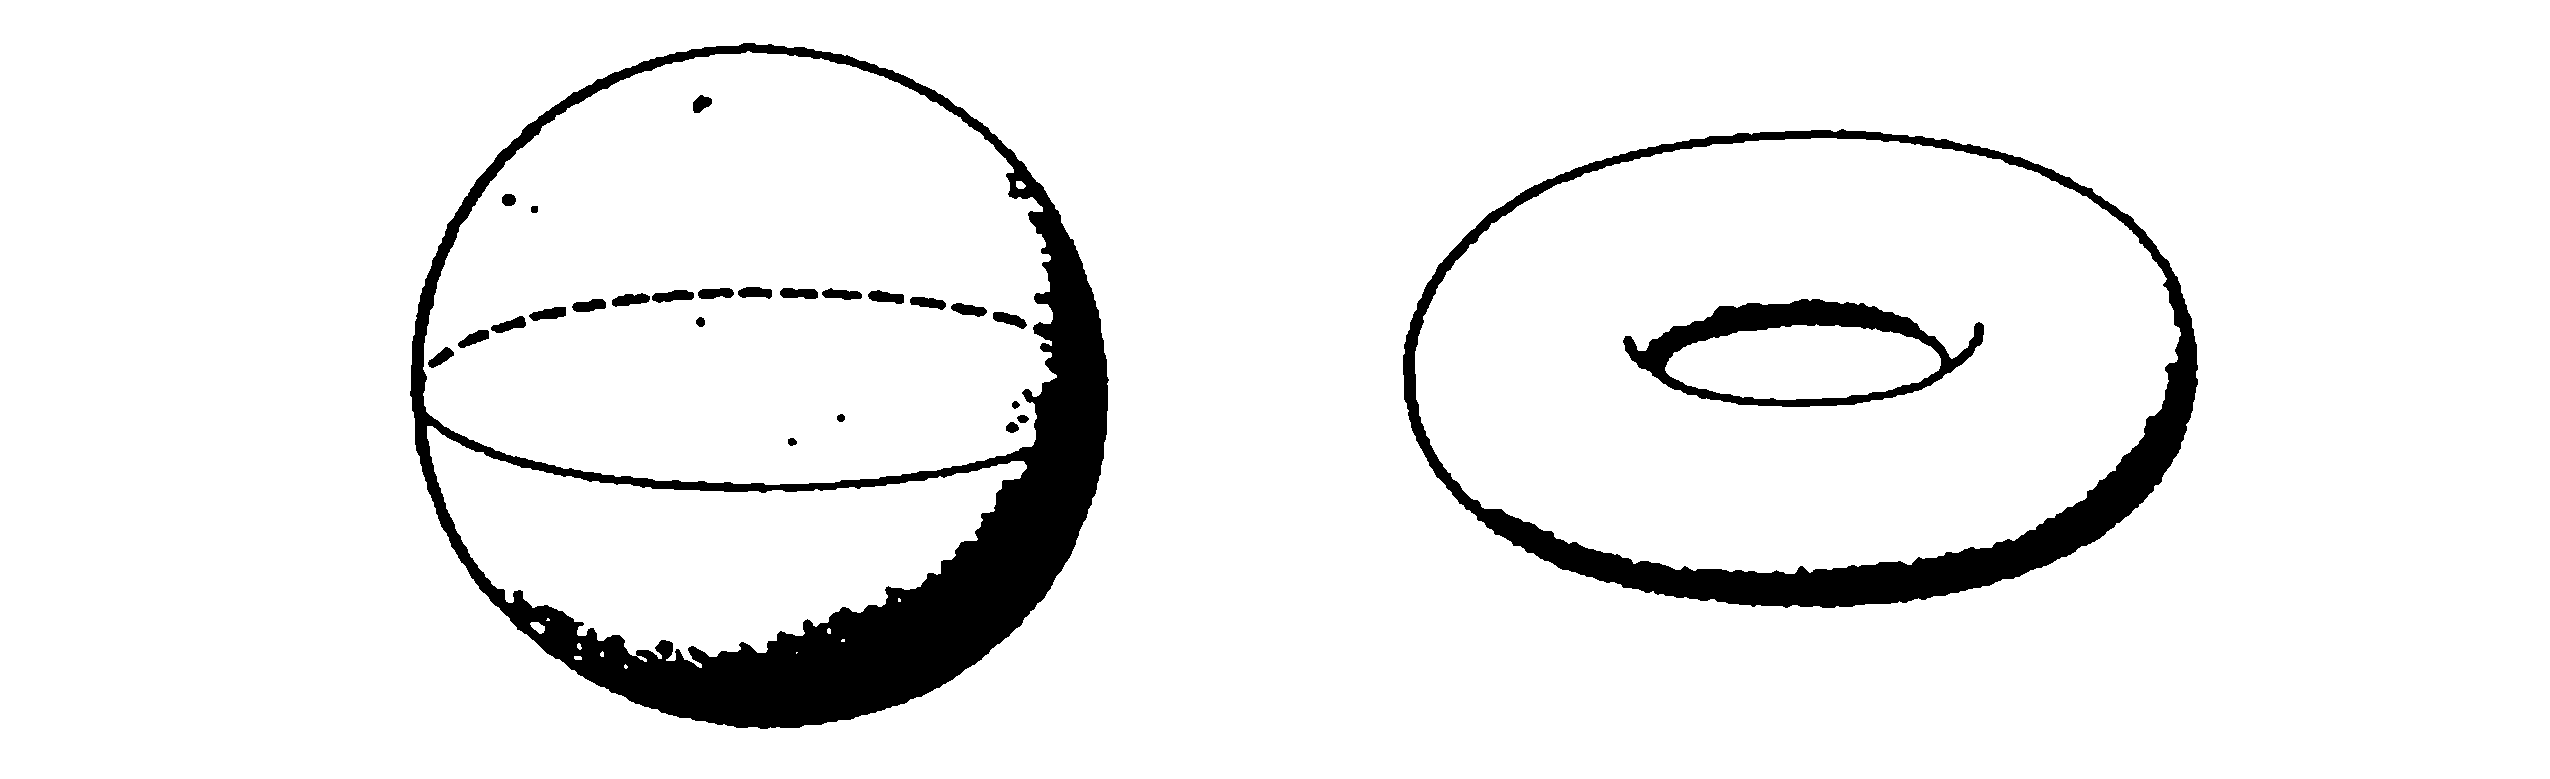
\includegraphics[width=\textwidth]{1-5.png}
\caption{Сфера и тор}
\label{fig:sphere_and_torus}
\end{figure}

Примеры \emph{замкнутых поверхностей} показаны на рисунках \ref{fig:sphere_and_torus} и \ref{fig:genus_2_3}: сфера и тор на рисунке \ref{fig:sphere_and_torus} и замкнутые поверхности рода два и три на рисунке \ref{fig:genus_2_3}. Нестрого говоря, \emph{род} поверхности --- это количество отверстий в ней. Род тора равен $1$, а род сферы равен $0$. Аналогично можно рассмотреть поверхность рода $g$ для любого натурального числа $g$.
% Далее сравнение с кругами для плавания от Michio Kuga, которое я опустил.

Будем обозначать сферу как $S^2$. Показатель $2$ указывает на размерность сферы. Тор будем обозначать как $T^2$. Также мы будем введём общее обозначение $\Sigma_g$ для замкнутой поверхности рода $g$, в этих обозначениях $\Sigma_0$ и $\Sigma_1$ есть не что иное, как сфера $S^2$ и тор $T^2$, соответственно.

\begin{figure}[ht]
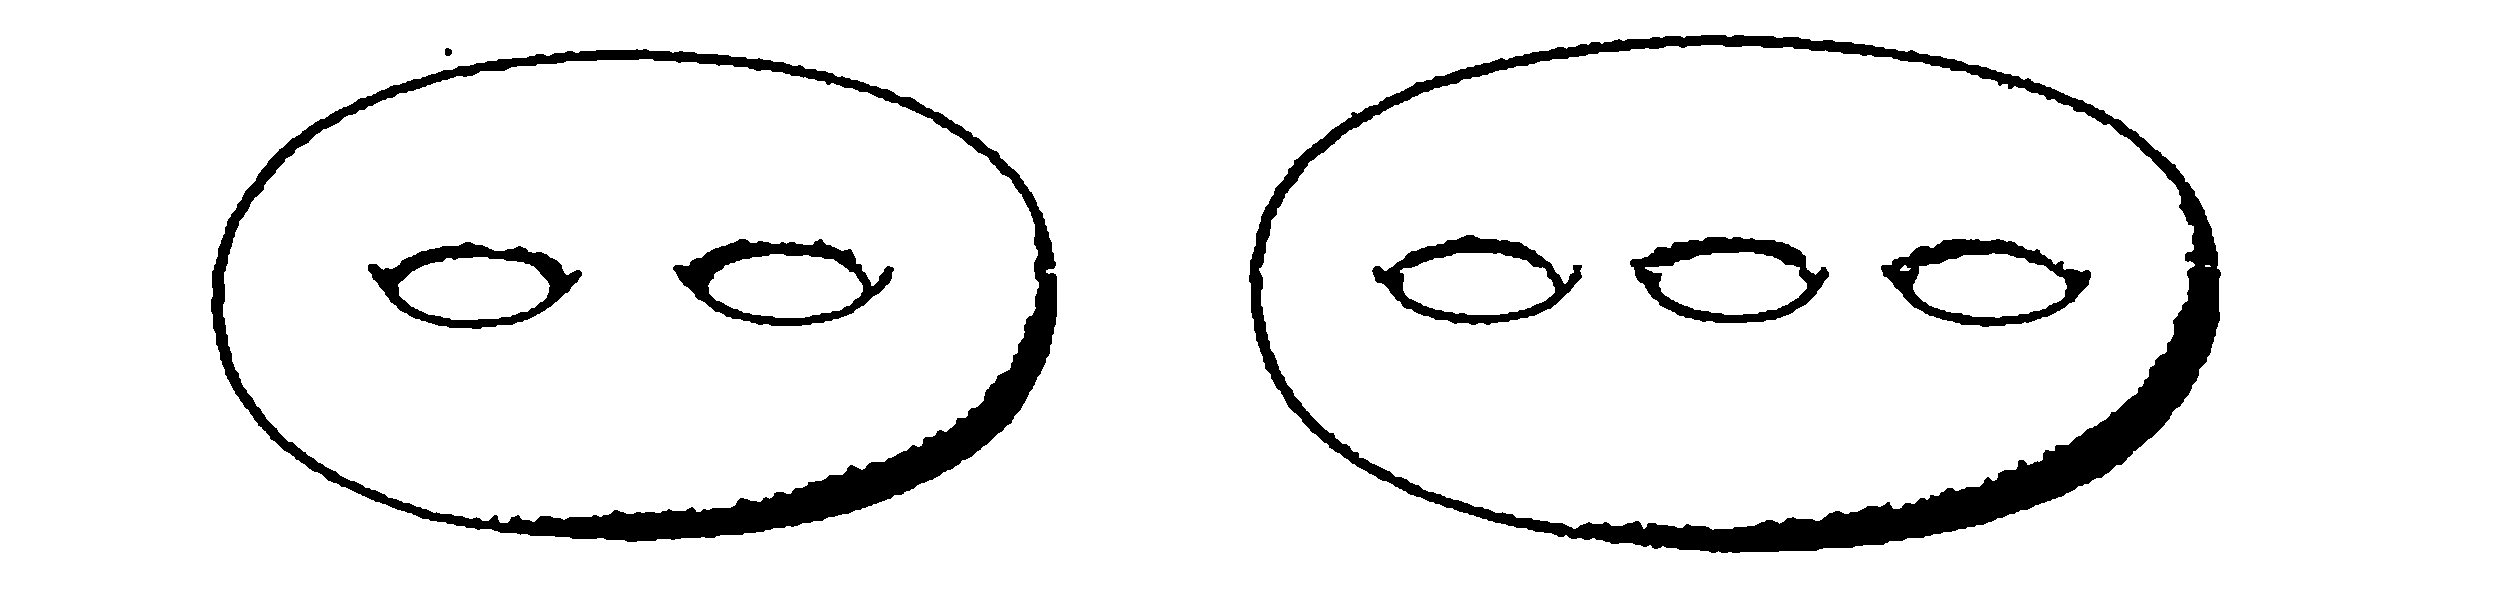
\includegraphics[width=\textwidth]{1-6.png}
\caption{Замкнутые поверхности рода 2 и 3}
\label{fig:genus_2_3}
\end{figure}

Пусть $M$ --- поверхность. Назовём отображение
\[
f:M \to \R,
\]
сопоставляющее каждой точке $p$ поверхности $M$ вещественное число, функцией на $M$.

Заметим, что локальные координаты на рассматриваемых поверхностях будут криволинейными (см. рисунок \ref{fig:surface_local_coords}).

\begin{figure}[ht]
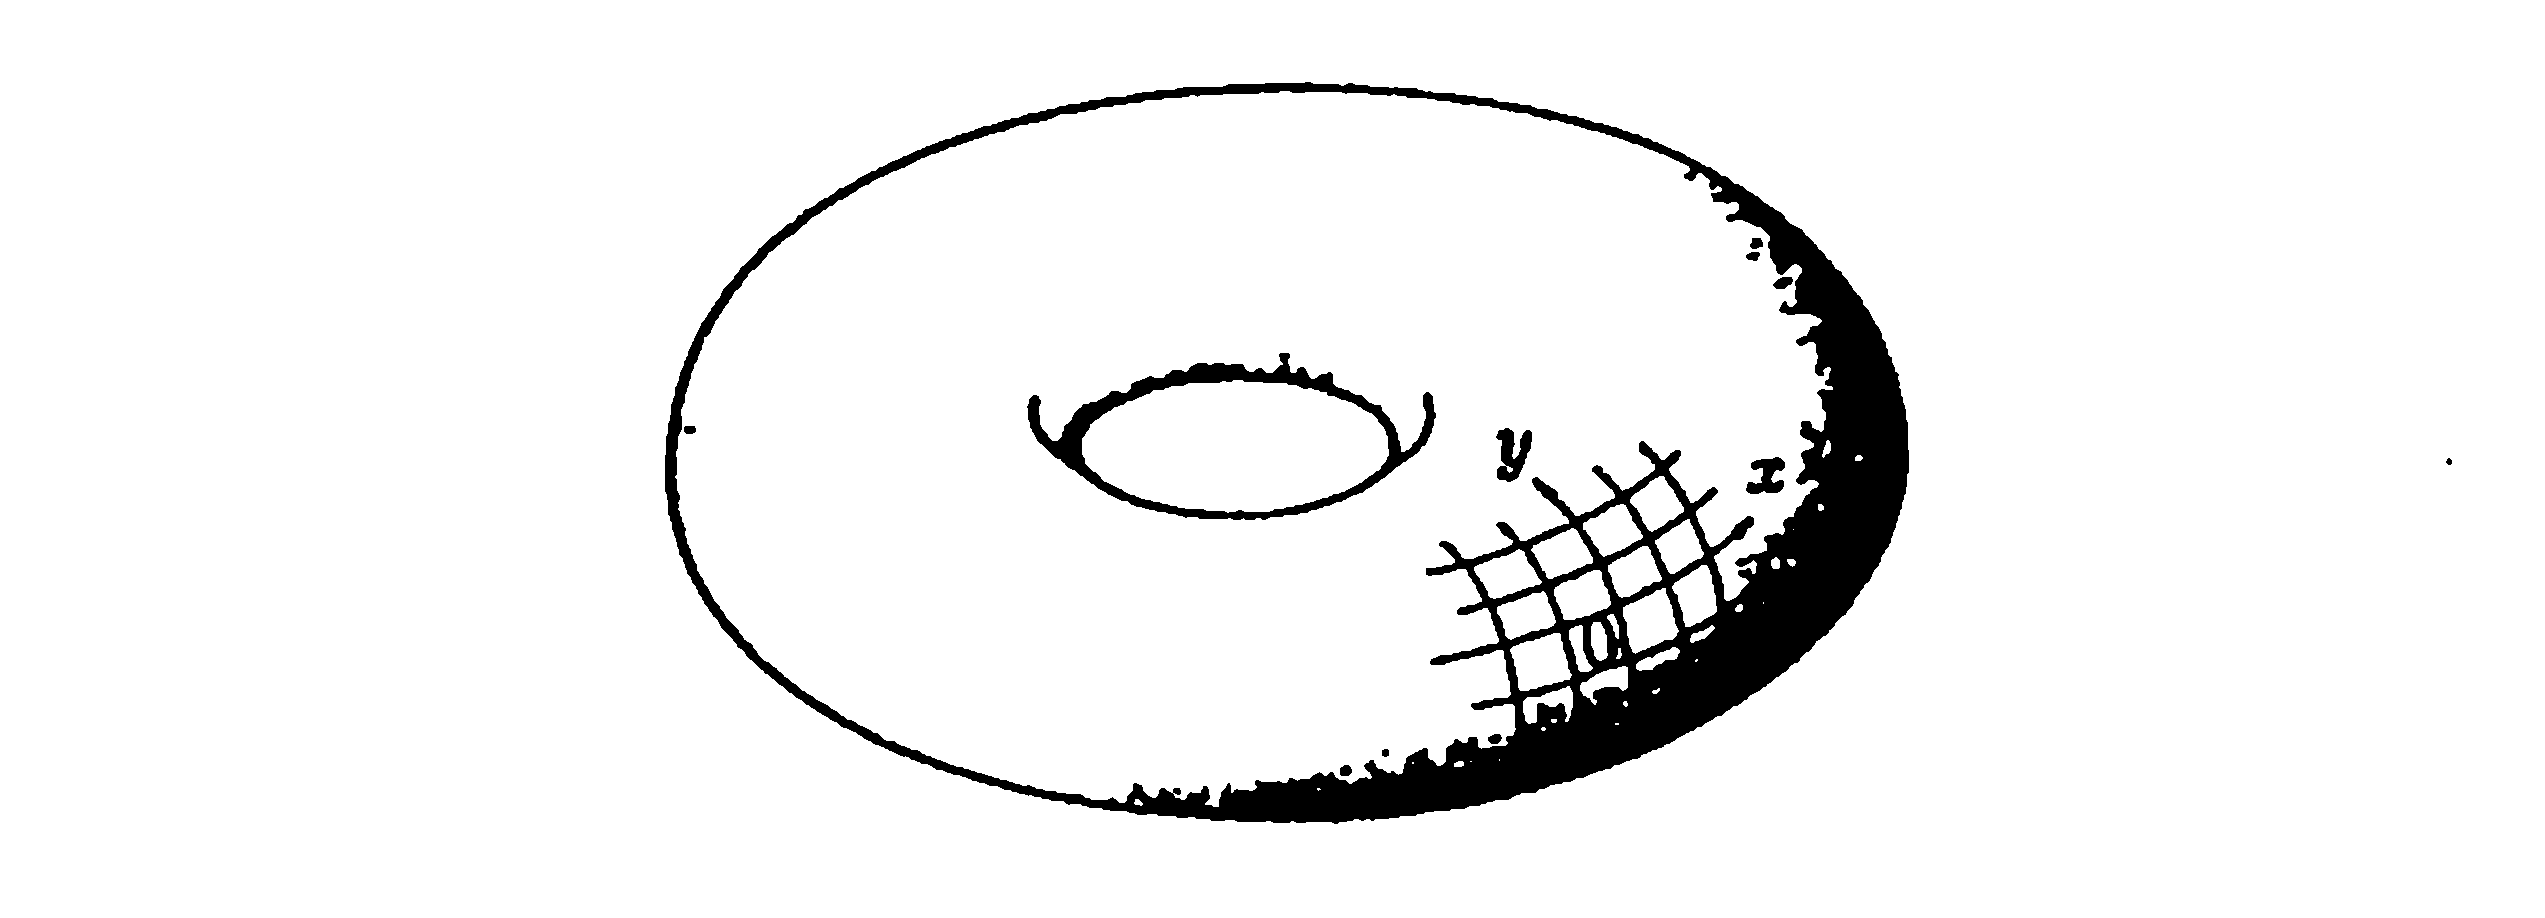
\includegraphics[width=\textwidth]{1-7.png}
\caption{Локальная система координат на торе}
\label{fig:surface_local_coords}
\end{figure}

Функция $f:M \to \R$ является гладкой (принадлежит классу $C^{\infty}$), если она принадлежит классу $C^{\infty}$ в любых гладких локальных координатах любой точки поверхности $M$.

С этого момента мы будем рассматривать только гладкие ($C^{\infty}$) поверхности и гладкие ($C^{\infty}$) функции на этих поверхностях.

Понятие критической точки, рассмотренное в предыдущем разделе, естественным образом обобщается на функцию $f:M \to \R$, определённую на поверхности $M$, при помощи локальных координат. А именно, точка $p_0$ поверхности $M$ называется \emph{критической точкой} функции $f:M \to \R$, если
\begin{equation}
\frac{\d f}{\d x}(p_0) = 0,\quad \frac{\d f}{\d y}(p_0) = 0
\label{eq:crit_point_surface}
\end{equation}
относительно локальных координат в некоторой окрестности точки $p_0$. Как мы видели в предыдущих разделах, невырожденные критические точки устойчивы и обладают некоторыми удобными свойствами, в отличие от вырожденных критических точек. Поэтому нам будет в дальнейшем рассматривать функции, обладающие только невырожденными критическими точками.

\begin{definition} (Функция Морса). Пусть все критические точки функции $f:M \to \R$ невырождены. Тогда скажем, что $f$ --- функция Морса.
\end{definition}

Рассмотрим несколько примеров таких функций.
    
\begin{figure}[ht]
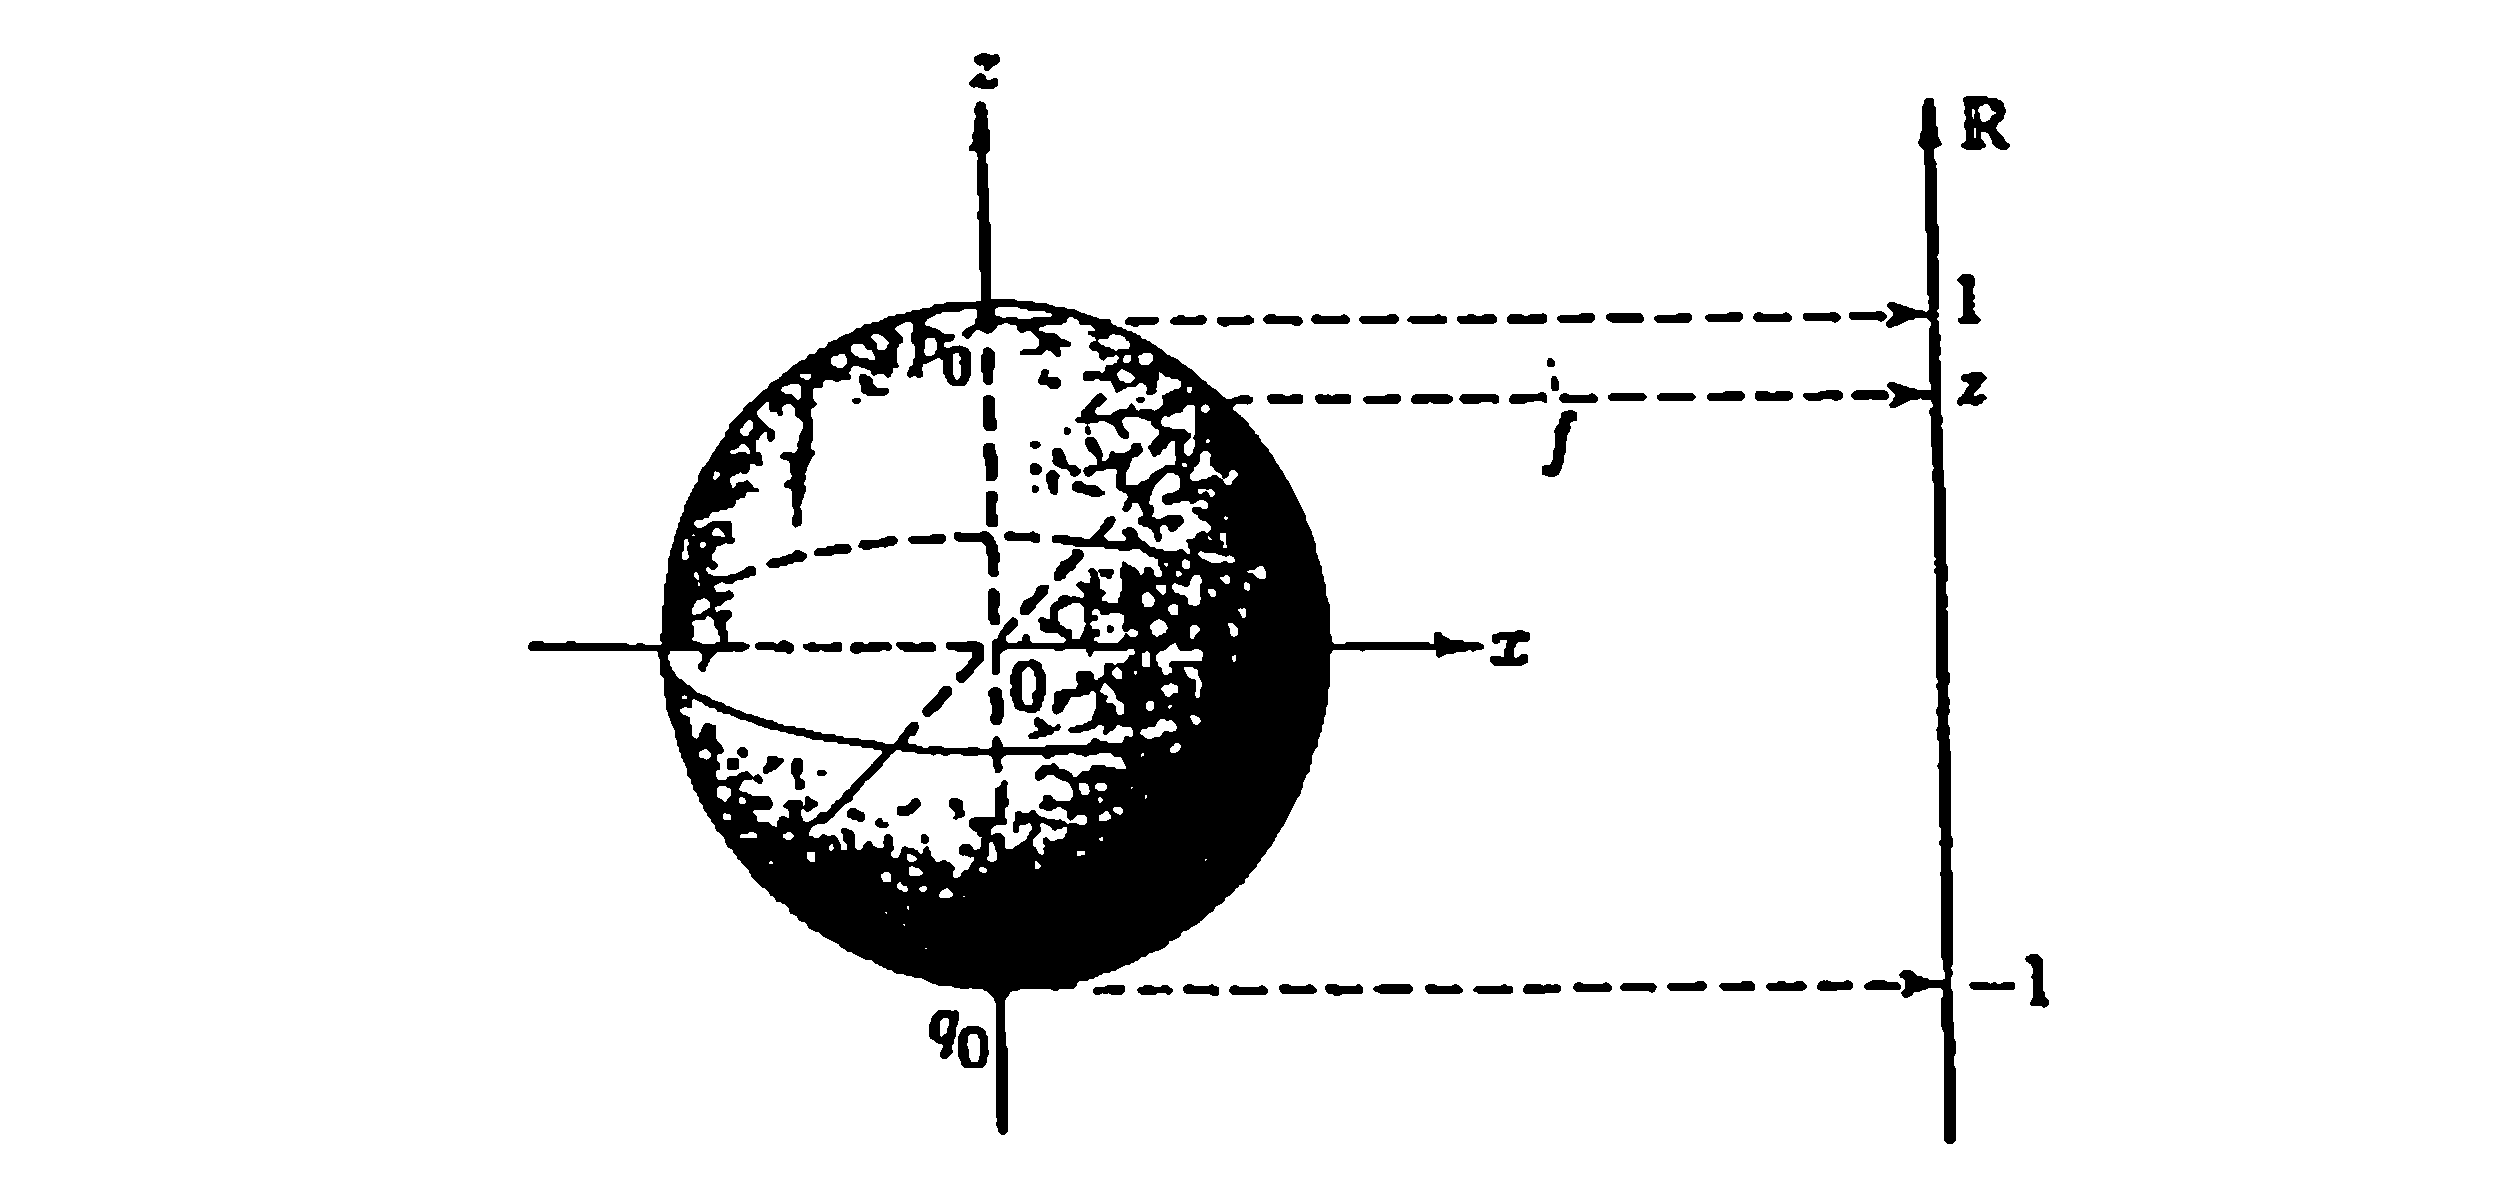
\includegraphics[width=\textwidth]{1-8.png}
\caption{Функция высоты на сфере}
\label{fig:sphere_height_function}
\end{figure}

\begin{example}(Функция высоты на сфере). Рассмотрим единичную сферу $S^2$ в декартовых координатах $(x, y, z)$ евклидова пространства $\R^3$; так, $S^2$ определена уравнением
\begin{equation}
x^2 + y^2 + z^2 = 1.
\end{equation}

Пусть $f:S^2 \to \R$ --- функция на $S^2$, сопоставляющая каждой точке $p = (x, y, z)$ сферы $S^2$ её координату $z$. Такую функцию можно назвать <<функцией высоты>>. Тогда $f$ является функцией Морса (рисунок \ref{fig:sphere_height_function}).

Действительно, у $f$ есть две критические точки: <<северный полюс>> $p_0 = (0, 0, 1)$ и <<южный полюс>> $q_0 = (0, 0, -1)$. Нетрудно заметить, что других критических точек на сфере нет. Чтобы проверить, что критические точки $p_0$ и $q_0$ невырожденные, достаточно вычислить гессиан функции $f$ относительно локальных координат $(x, y)$ --- он будет ненулевым.
\end{example}

В данном примере мы рассмотрели функцию Морса на сфере с ровно двумя критическими точками, обе из которых невырождены. Оказывается, верно обратное.

\begin{theorem}
Пусть $M$ --- замкнутая поверхность, $f:M\to\R$ --- функция Морса с ровно двумя невырожденными критическими точками (других критических точек нет). Тогда $M$ диффеоморфна сфере $S^2$.
\label{thm:sphere_2d}
\end{theorem}

Эта теорема --- простой пример применения теории Морса. Перед тем, как доказывать теорему, определим понятие <<диффеоморфизм>>.

Начнём с понятия <<гомеоморфизма>>. Пусть дано взаимно однозначное отображение
\[
h: X \to Y
\]
между двумя (топологическими) пространствами $X$ и $Y$. Мы можем определить обратное отображение
\[
h^{-1}: Y \to X.
\]
Если оба отображения $h: X \to Y$ и $h^{-1}: Y \to X$ непрерывны, то отображение $h$ называется \emph{гомеоморфизмом}. Два (топологических) пространства называются \emph{гомеоморфными}, если существует гомеоморфизм между ними. В топологии пространства часто рассматриваются <<с точностью до гомеоморфизма>>, т. е. гомеоморфные пространства считаются одинаковыми, <<имеющими одну и ту же форму>>.

\begin{definition}
Гомеоморфизм
\[
h:M\to N
\]
между поверхностями $M$ и $N$ называется \emph{диффеоморфизмом}, если отображения $h: M \to N$ и $h^{-1}: N \to M$ принадлежат классу $C^{\infty}$. Поверхности $M$ и $N$ называются \emph{диффеоморфными}, если между ними существует диффеоморфизм.
\end{definition}

Диффеоморфные поверхности рассматриваются как имеющие одинаковую форму и гладкую структуру. В дифференциальной топологии, где объектами изучения являются гладкие геометрические фигуры, пространства рассматриваются <<с точностью до диффеоморфизма>>.

Теперь докажем Теорему \ref{thm:sphere_2d} (см. рисунок \ref{fig:diffeomorphic}).

\begin{figure}[ht]
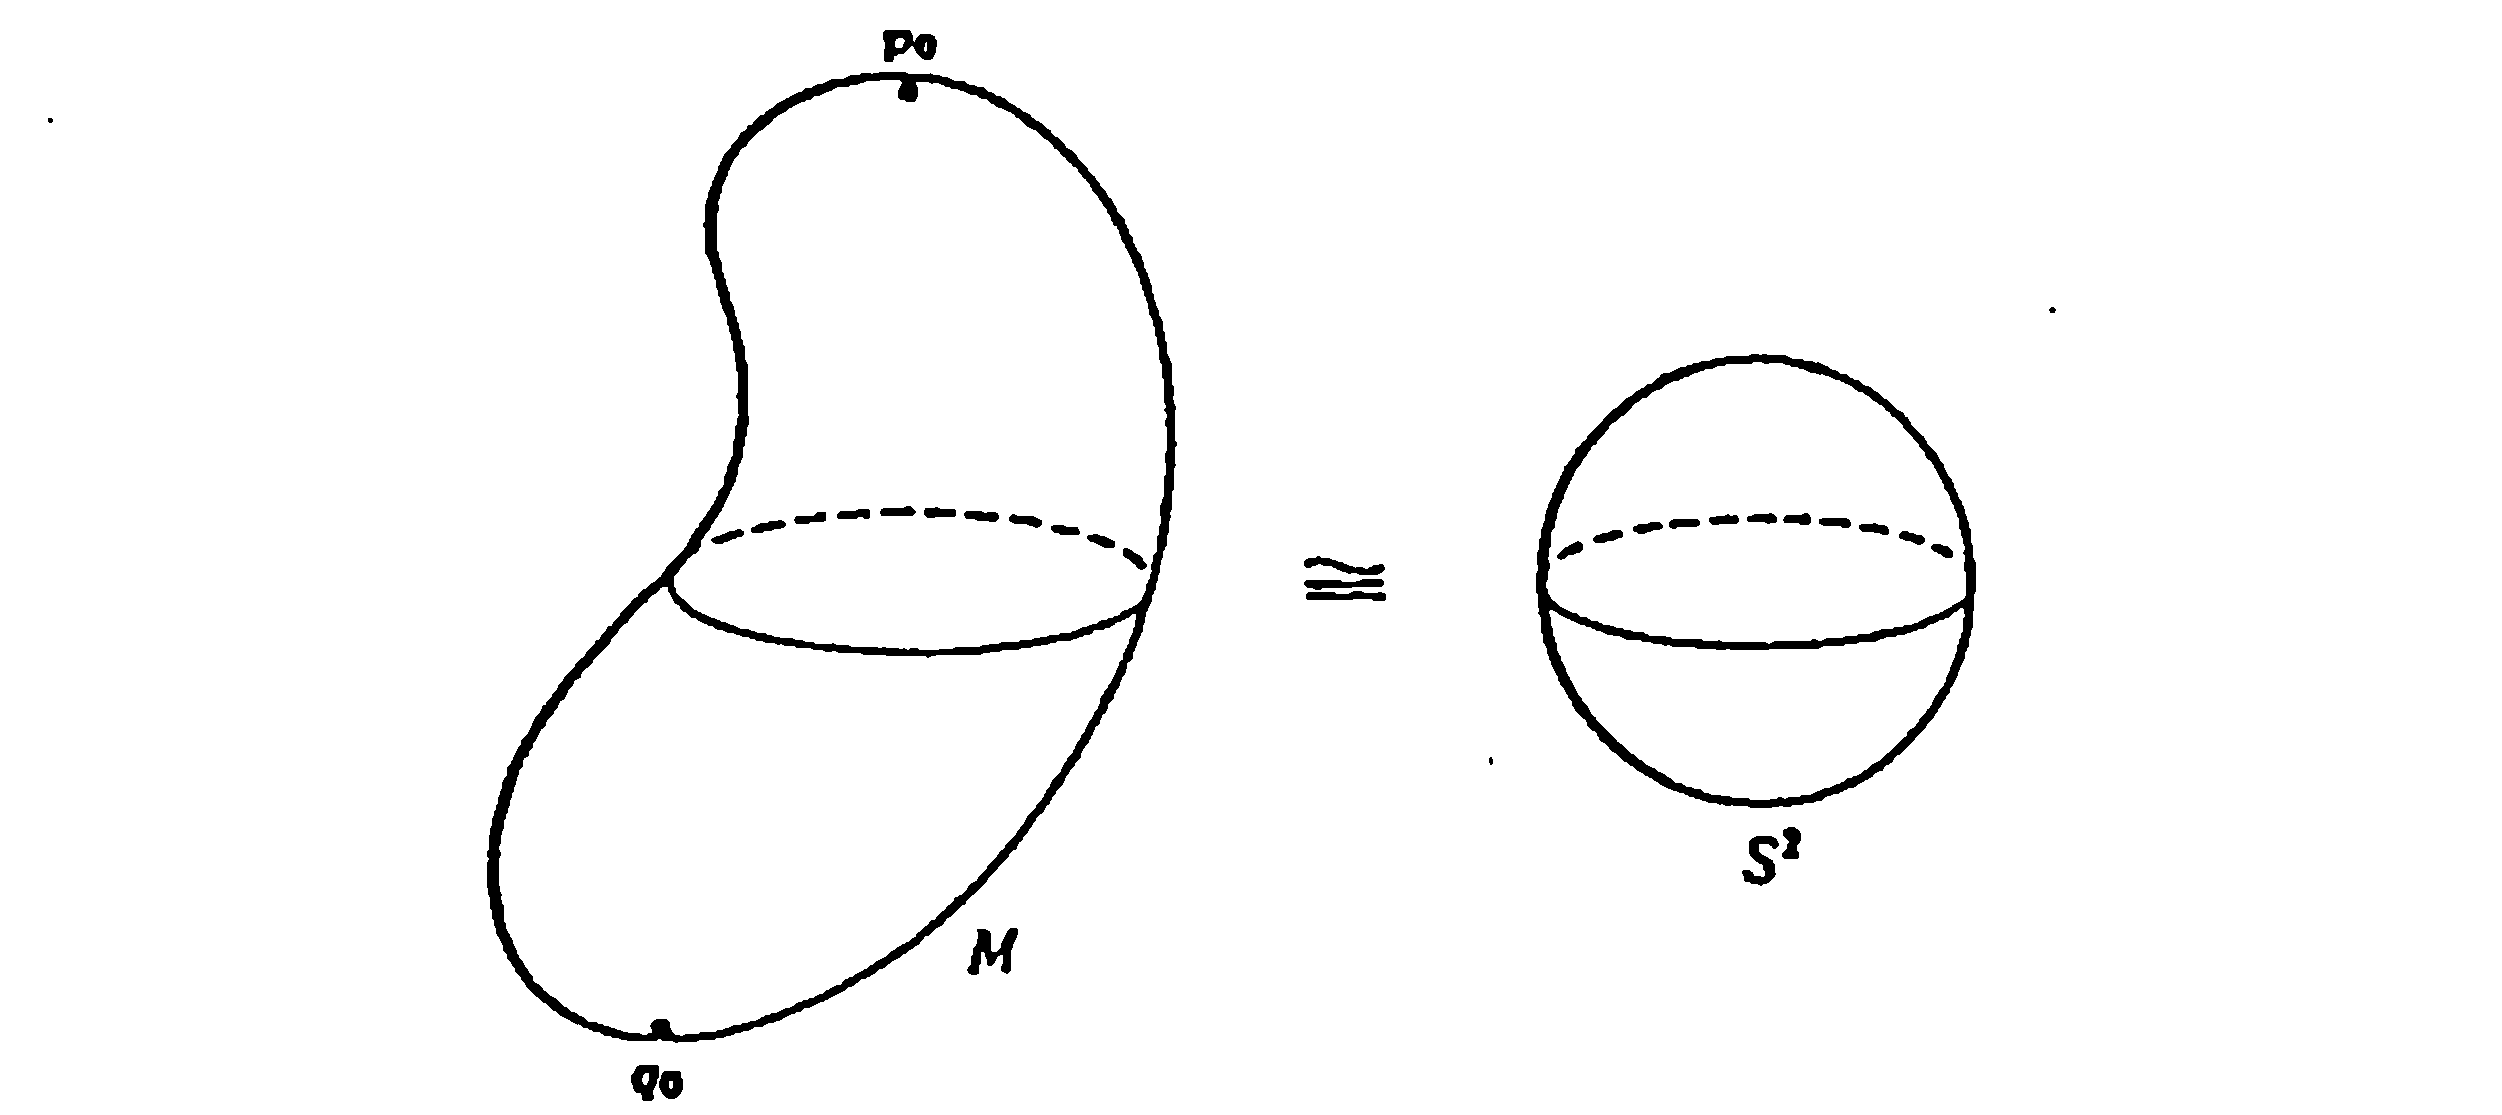
\includegraphics[width=\textwidth]{1-9.png}
\caption{Поверхность $M$ диффеоморфна сфере $S^2$}
\label{fig:diffeomorphic}
\end{figure}

\begin{proof}
Заметим, что замкнутая поверхность является компактом (на самом деле, замкнутая поверхность определяется как <<двумерное компактное многообразия без края>>). Подробнее это понятие будет рассмотрено во 2-й главе. В ходе доказательства мы будем пользоваться теоремой Вейерштрасса о непрерывной функции на компакте:

\begin{theorem} (Теорема Вейерштрасса о максимальном значении). Пусть $f: X \to \R$ --- непрерывная функция на компакте $X$. Тогда $f$ принимает максимальное значение в некоторой точке $p_0 \in X$ и минимальное значение в некоторой точке $q_0 \in X$.
\end{theorem}

Этот факт достаточно известен, поэтому здесь мы опустим его доказательство.

По теореме Вейерштрасса, функция Морса $f:M\to \R$ принимает максимальное значение в некоторой точке $p_0 \in M$ и минимальное значение в некоторой (другой) точке $q_0 \in M$. Точки $p_0$ и $q_0$ --- критические точки функции $f$. Более того, поскольку $f$ --- функция Морса, $p_0$ и $q_0$ --- невырожденные критические точки.

По лемме Морса (Теорема \ref{thm:morse_lemma_2d}, функцию $f$ можно представить в стандартной форме в подходящих локальных координатах $(x, y)$ в окрестности точки $p_0$ и координатах $(X, Y)$ в окрестности точки $q_0$.

Поскольку $p_0$ --- максимум, индекс $p_0$ равен $2$; поскольку $q_0$ --- минимум, индекс $q_0$ равен $0$. Следовательно, имеем два представления в окрестности критических точек:
\begin{equation}
f =
\begin{cases}
-x^2 - y^2 + A & (\text{в окрестности }p_0),\\
X^2 + Y^2 + a & (\text{в окрестности }q_0),
\end{cases}
\label{eq:bowls}
\end{equation}
где $A = f(p_0)$, $a = f(q_0)$.

Пусть $\epsilon$ --- достаточно малое положительное число. Обозначим как $D(p_0)$ окрестность точки $p_0$, для точек $p$ из которой
\begin{equation}
A - \epsilon \leq f(p) \leq A.
\end{equation}

\begin{figure}[t]

\includegraphics[width=\textwidth]{1-10.png}
\caption{Слева: график $f$ в окрестности $p_0$; справа: график $f$ в окрестности $q_0$.}
\label{fig:bowls}
\end{figure}

<<Перевёрнутая чаша>> параболоида слева на рисунке \ref{fig:bowls} соответствует множеству $D(p_0)$ которое в координатах $(x, y)$ характеризуется уравнением
\begin{equation}
x^2 + y^2 \leq \epsilon,
\label{eq:2disk}
\end{equation}
как видно из равенства (\ref{eq:bowls}). Другими словами, $D(p_0)$ диффеоморфно $2$-диску (двумерному диску), определённому уравнением (\ref{eq:2disk}). Аналогично, множество $D(q_0)$ точек окрестности $q_0$, удовлетворяющих неравенству
\begin{equation}
a \leq f(p) \leq a + \epsilon,
\end{equation}

соответствует чаше параболоида справа на рисунке \ref{fig:bowls}. В координатах (X, Y) множество $D(q_0)$ принимает вид
\begin{equation}
X^2 + Y^2 \leq \epsilon,
\label{eq:2disk2}
\end{equation}
и также диффеоморфно $2$-диску.

Удалим внутренность дисков $D(p_0)$ и $D(q_0)$ из поверхности $M$, оставшуюся поверхность с краем обозначим как $M_0$. Граница $M_0$ состоит из граничных окружностей $C(p_0)$ и $C(q_0)$ дисков $D(p_0)$ и $D(q_0)$, соответственно.

В общем случае, граница поверхности с краем $M_0$ обозначается как
\begin{equation}
\d M_0.
\end{equation}

В нашем случае граница состоит из двух окружностей $C(p_0)$ и $C(q_0)$, поэтому мы можем записать:
\begin{equation}
\d M_0 = C(p_0) \cup C(q_0).
\end{equation}

Будем обозначать как
\begin{equation}
\inter(M_0)
\end{equation}
\emph{внутренность} $M_0$ --- то, что останется после удаления границы из $M_0$. По определению, $\inter(M_0) = M_0 \setminus \d M_0$.

\begin{figure}[t]
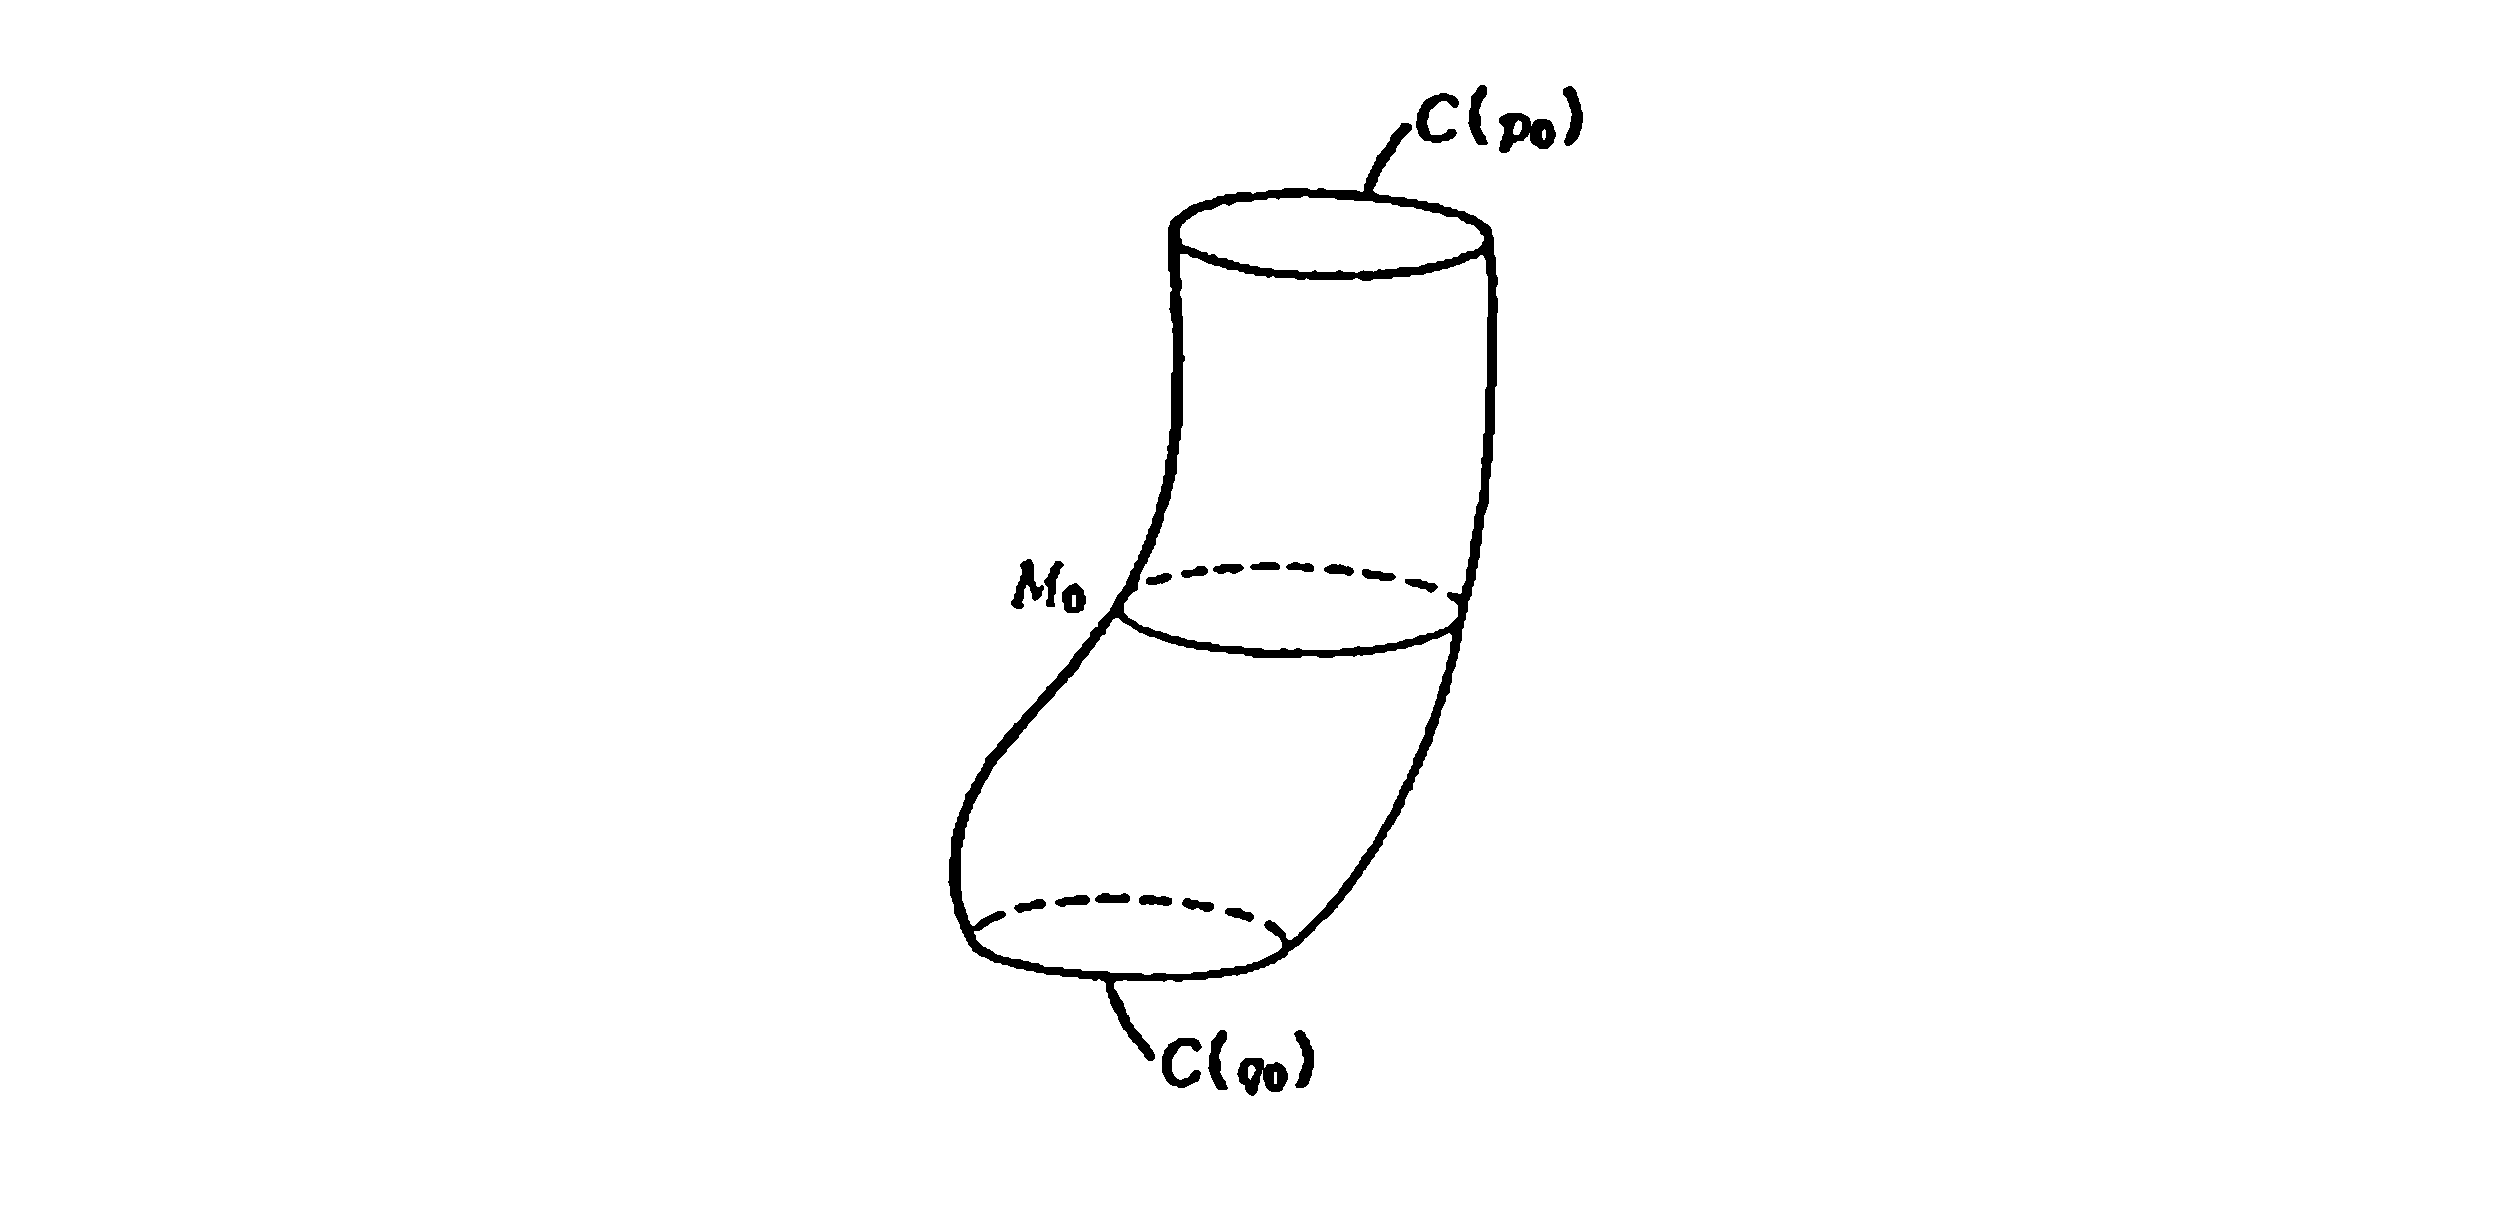
\includegraphics[width=\textwidth]{1-11.png}
\caption{Поверхность $M_0$.}
\label{fig:m0_surface}
\end{figure}

Из определения $D(p_0)$ и $D(q_0)$ очевидно, что ограничение функции $f$ на $M_0$, $f: M_0 \to \R$, принимает постоянные значения $A - \epsilon$ и $a + \epsilon$ на граничных окружностях $C(p_0)$ и $C(q_0)$, соответственно.

Напомним, что по условию Теоремы \ref{thm:sphere_2d} рассматриваемая функция Морса имеет ровно две критические точки. Поэтому после удаления (внутренности) $D(p_0)$ и $D(q_0)$ у функции $f: M_0 \to \R$ критических точек не останется. Сформулируем факт, которым мы сейчас воспользуемся, а докажем позднее (TODO) в более общем виде.

\begin{lemma}
Пусть $f: M_0 \to \R$ --- функция класса $C^{\infty}$, которая является константой на граничных окружностях $C(p_0)$ и $C(q_0)$. Также пусть у $f$ нет критических точек на $M_0$. Тогда $M_0$ диффеоморфна прямому произведению окружности на единичный отрезок, т.~е. $M_0 \cong C(q_0) \times [0, 1]$.
\label{lm:cylinder_2d}
\end{lemma}

Поскольку $C(p_0)$ и $C(q_0)$ диффеоморфны единичной окружности (обозначаемой $S^1$), из Леммы \ref{lm:cylinder_2d} следует, что $M_0$ диффеоморфна прямому произведению
\[
S^1 \times [0, 1].
\]

Вообще, поверхность, диффеоморфная прямому произведению $S^1 \times [0, 1]$ называется \emph{кольцом} (в топологическом, а не алгебраическом смысле). Так, если удалить из диска $\Delta$ внутренность меньшего концентрического диска $\Delta_0$, полученная поверхность $A$ будет являться кольцом.

По Лемме \ref{lm:cylinder_2d}, $M_0$ --- кольцо. Пусть
\[
N_0 = M_0 \cup D(q_0);
\]

так, $N_0$ --- это объединение $M_0$ с чашей гиперболоида. Точнее, $N_0$ получается приклейкой диска $D(q_0)$ к $M_0$ по граничной окружности $C(q_0)$, и поэтому поверхность $N_0$ тоже диффеоморфна диску.

Теперь приклеим диск $D(p_0)$ по граничной окружности к $N_0$ (у них общая граница) так, чтобы снова получить поверхность $M$. Таким образом, мы получили поверхность $M$ склейкой двух дисков по границе, откуда следует, что $M$ диффеоморфна сфере $S^2$.
\end{proof}

Строго говоря, нам нужна следующая лемма (Упражнение TODO), чтобы показать, что замкнутая поверхность, образованная склейкой двух дисков по границе диффеоморфна сфере $S^2$.

\begin{lemma}
Пусть отображение
\begin{equation}
k: \d D_0 \to \d D_1
\end{equation}
является диффеоморфизмом между границами дисков $D_0$ и $D_1$, соответственно. Тогда мы можем продолжить $k$ до диффеоморфизма дисков
\begin{equation}
K:D_0 \to D_1.
\end{equation}
\label{lm:diff_extension_disk}
\end{lemma}

Доказательство леммы смотрите в Упражнении (TODO). Подчеркнём, что утверждение леммы не является очевидным. На самом деле, оно выполняется для дисков размерности, не превышающей $6$, а для больших размерностей, вообще, неверно.

В заключение раздела докажем следующий базовый факт.

\begin{lemma}
Функция Морса $f:M \to \R$, определённая на замкнутой поверхности $M$, имеет конечное количество критических точек.
\label{lm:finite_crit_pts_2d}
\end{lemma}

\begin{proof}
Предположим, что у функции Морса $f: M \to \R$ бесконечно много критических точек
\[p_1, p_2, p_3, \ldots\]
Поскольку $M$ --- компакт, существует сходящаяся подпоследовательность $p_{n_1}, p_{n_2}, \ldots$ данной последовательности. Пусть $p_0$ --- предел этой подпоследовательности. Не ограничивая общности, будем считать, что вся последовательность $\{p_{n_i}\}_{i = 1}^{\infty}$ содержится внутри окрестности $U$ точки $p_0$.

Поскольку функция $f$ гладкая, её производные $\dfrac{\d f}{\d x}(p)$ и $\dfrac{\d f}{\d y}(p)$ непрерывно зависят от $p$. Производные $\dfrac{\d f}{\d x}(p)$ и $\dfrac{\d f}{\d y}(p)$ принимают нулевое значение в точках последовательности $p_{n_1}, p_{n_2}, \ldots$. Следовательно, в предельной точке $p_0$ производные также равны нулю, значит, $p_0$ --- критическая точка функции $f$. Но в любой окрестности критической точки $p_0$ содержится бесконечное число других критических точек, что противоречит утверждению (Следствие \ref{corol:crit_points_isolated_2d}) об изолированности критических точек. Это противоречие завершает доказательство Леммы \ref{lm:finite_crit_pts_2d}.
\end{proof}

\section{Разложение на ручки}

В Теореме \ref{thm:sphere_2d} мы показали, что в одном частном случае функция Морса может определять форму поверхности, на которой она определена. Предмет теории Морса (в особенности, теории Морса для конечномерных пространств) заключается в изучении этого явления. В этом разделе мы опишем важный инструмент для изучения формы поверхности --- <<разложение на ручки>>.

Пусть
\[f:M\to\R\]
--- функция морса, определённая на замкнутой поверхности.

Далее мы будем считать замкнутую поверхность $M$ \emph{связной}. Для поверхности $M$ (а в общем случае, для многообразия $M$), это предположение означает то же, что и \emph{линейная связность}, т.~е. любые две точки $p$ и $q$ поверхности $M$ соединены кривой, лежащей на $M$.

\begin{figure}[t]
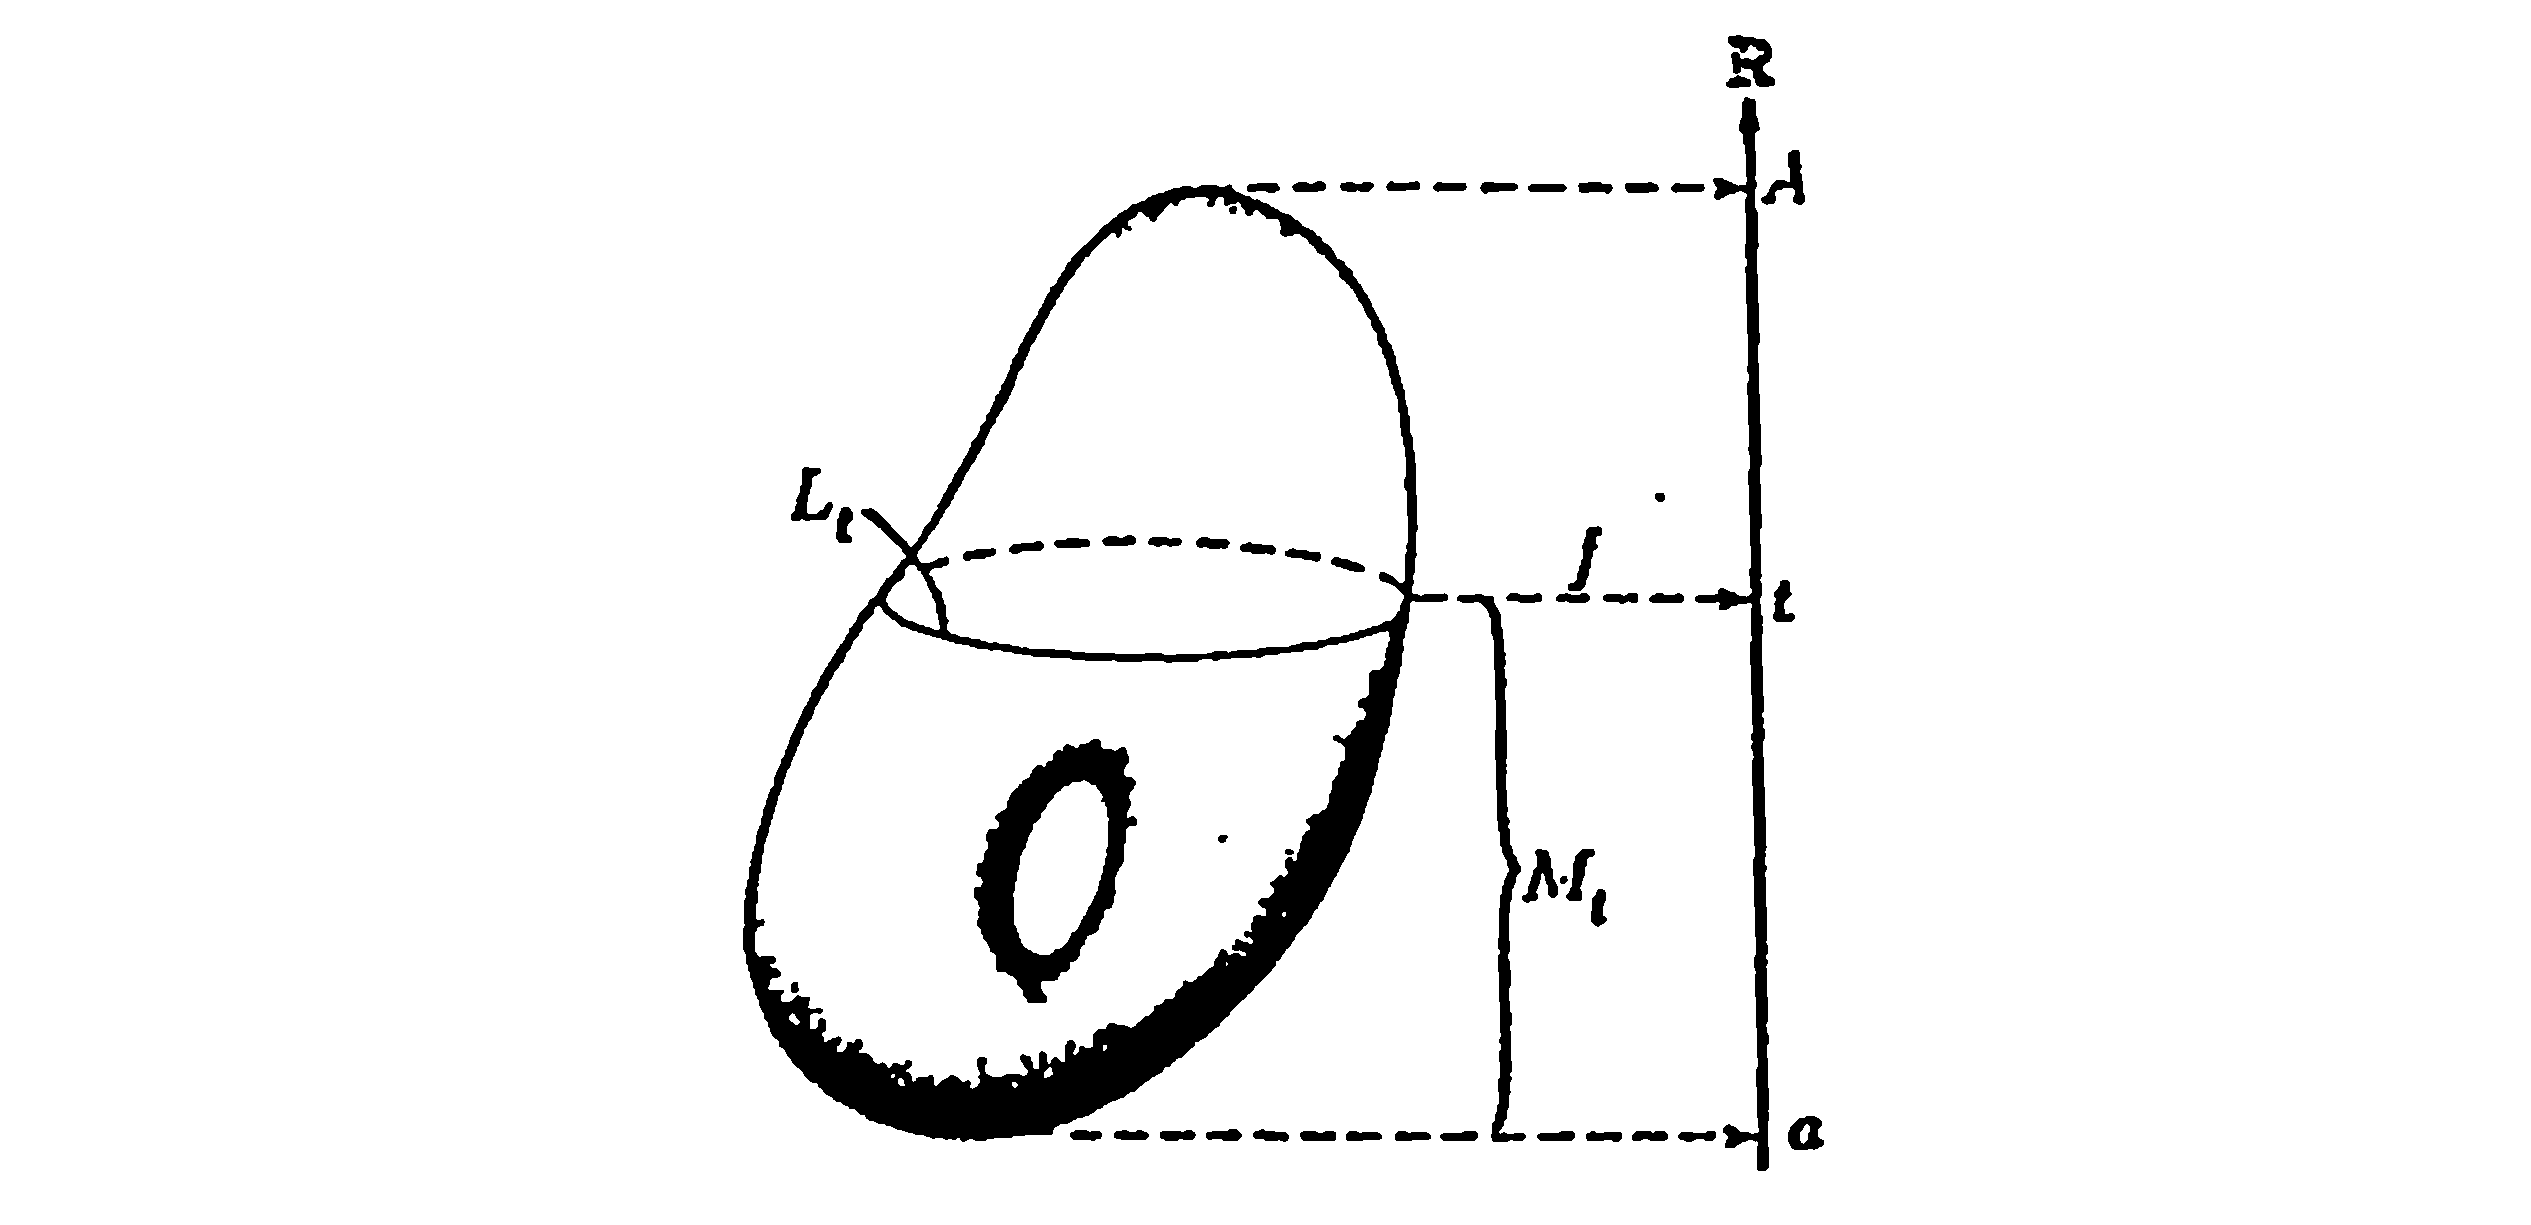
\includegraphics[width=\textwidth]{1-12.png}
\caption{Множество подуровня $M_t$ и кривая уровня $L_t$.}
\label{fig:sublevel_surface}
\end{figure}

Для функции Морса $f: M \to \R$ мы будем обозначать как $M_t$ \emph{множество подуровня} $M$ состоящее из точек, в которых функция $f$ принимает значения, меньшие или равные вещественного числа $t$:
\begin{equation}
M_t = \{p \in M \,\mid\,f(p)\leq t\}.
\end{equation}
Обозначим как $L_t$ \emph{кривую уровня} (или \emph{множество уровня}) функции $f$, т. е. множество точек, в которых функция $f$ принимает значение $t$.

Пусть $f$ принимает на $M$ максимальное значение $A$ и минимальное значение $a$. Поскольку не существует точек $p$, для которых $f(p) < a$,
\[M_t = \emptyset\]
при $t < a$. Также заметим, что $f(p) \leq A$ в любой точке $p \in M$, поэтому $f(p) \leq t$ при $t \geq A$; значит, при $t \geq A$
\[M_t = M.\]
Следовательно, при изменении параметра $t$ в интервале от $a$ до $A$, множество подуровня $M_t$ изменяется от пустого множества до всей поверхности $M$. Фундаментальная идея теории Морса состоит в описании изменения формы множества подуровня $M_t$ в зависимости от $t$.

Можно представить ситуацию так, что $f: M \to \R$ --- функция высоты, и мы погружаем $M$ в воду. Параметр $t$ соответствует уровню воды, а $M_t$ --- часть $M$, ушедшая под воду, при уровне воды $t$. При увеличении уровня $t$ форма <<подводной>> части изменяется. Теория Морса изучает изменение формы множества $M_t$, расположенного <<под водой>>.

\begin{definition} (Критические значения). Вещественное число $c_0$ называется критическим значением функции $f$, если $f$ принимает значение $c_0$ в некоторой критической точке $p_0$: $f(p_0) = c_0$.
\end{definition}

\begin{figure}[t]
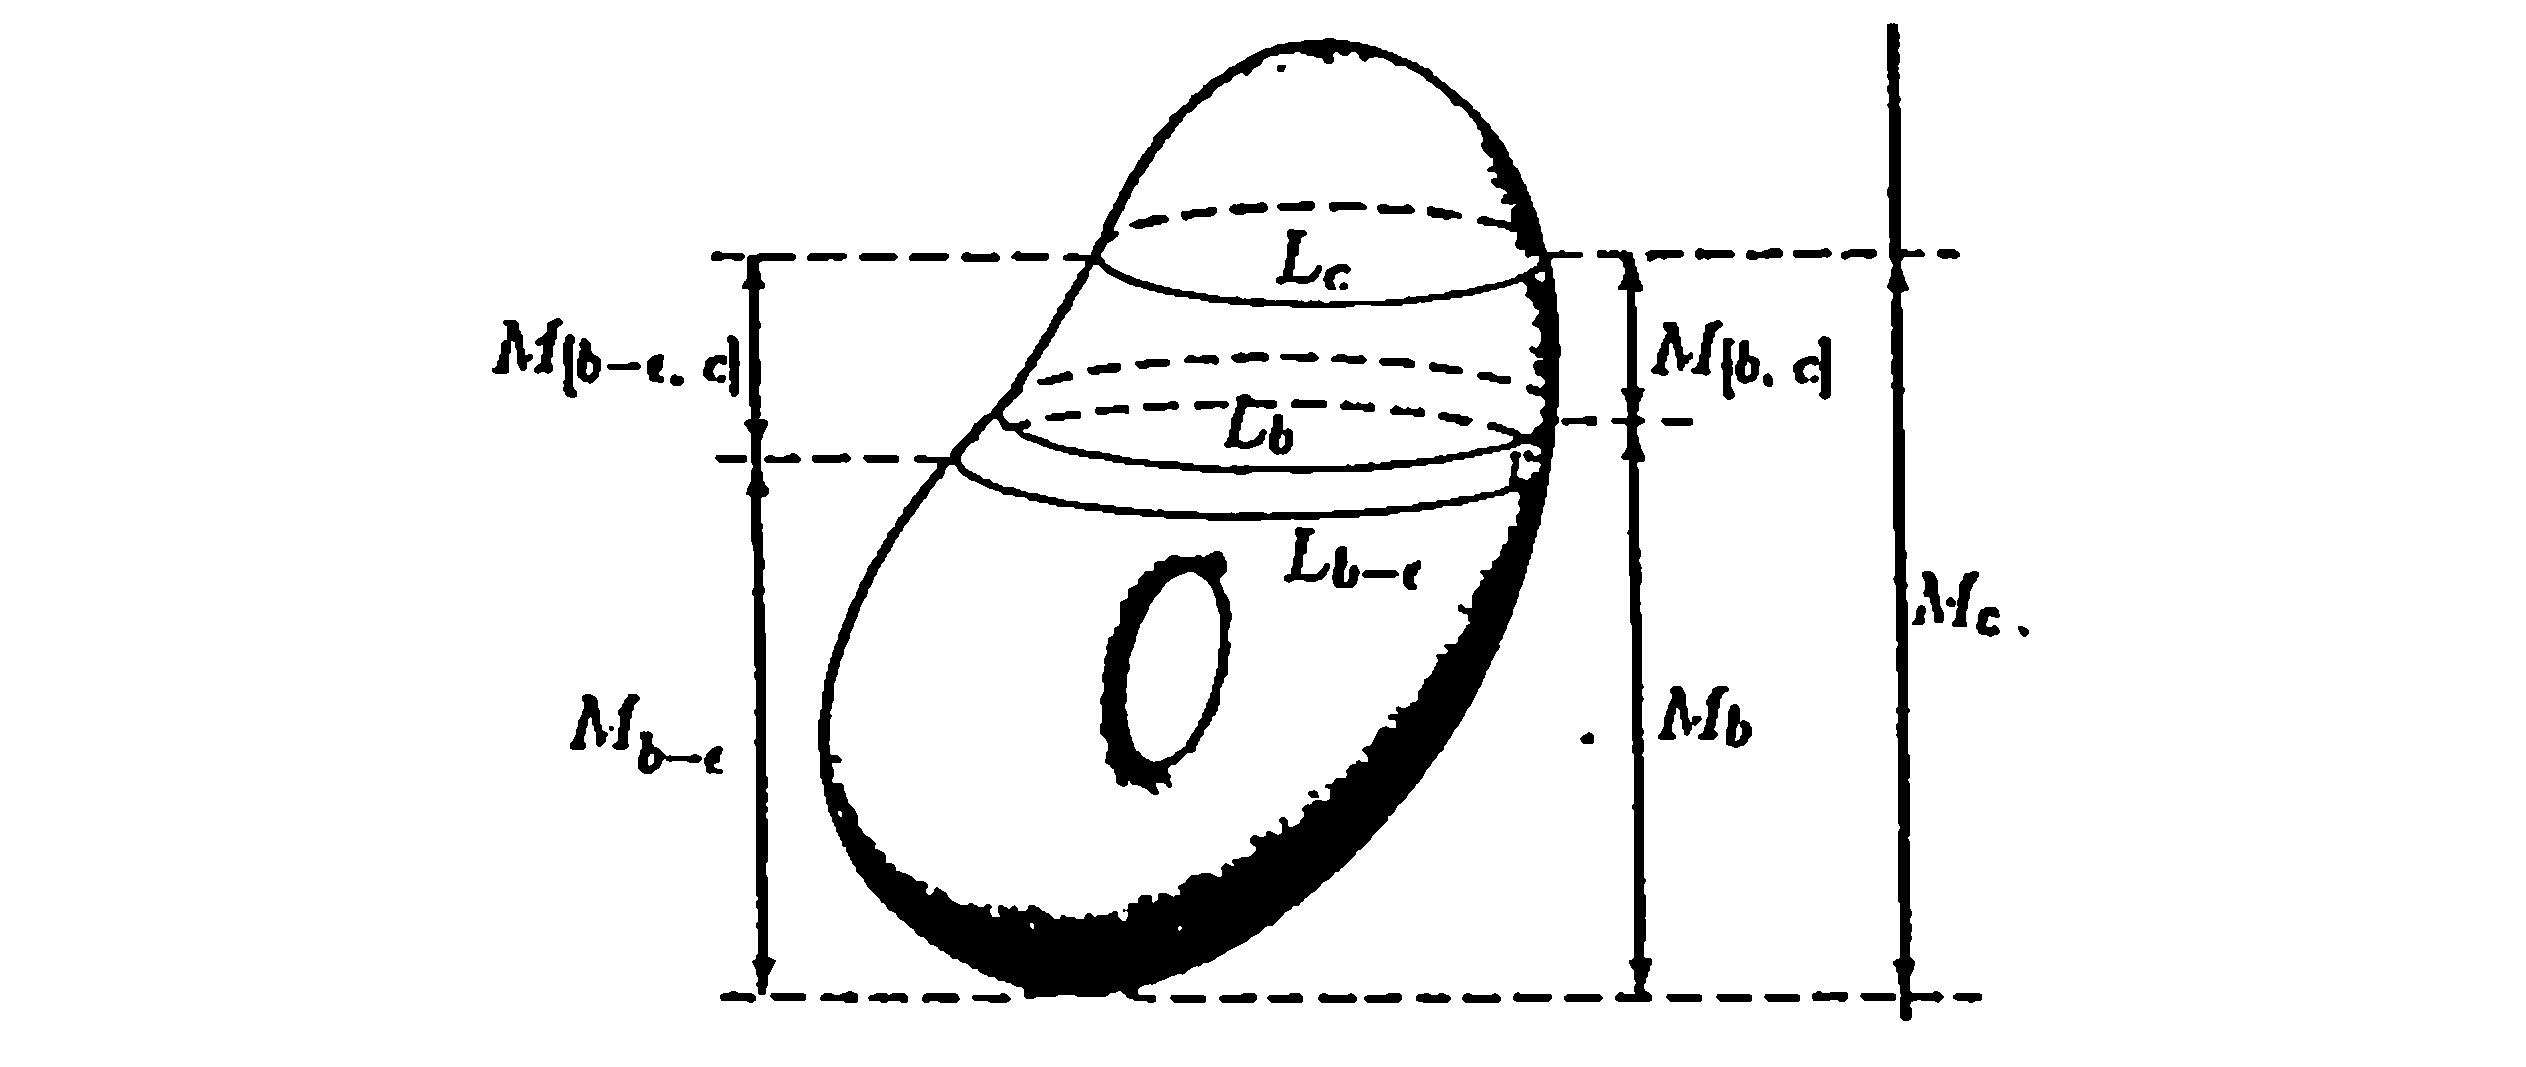
\includegraphics[width=\textwidth]{1-13.png}
\caption{Между $L_b$ и $L_c$ нет критических точек.}
\label{fig:lemma_cylinder}
\end{figure}

\begin{lemma}
Пусть $b < c$ --- вещественные числа такие, что у $f$ нет критических значений на отрезке $[b, c]$. Тогда множества $M_b$ и $M_c$ диффеоморфны (см. рисунок \ref{fig:lemma_cylinder}).
\label{lm:lemma_cylinder}
\end{lemma}

\begin{proof}
Поскольку максимальное и минимальное значения, $A$ и $a$, соответственно, являются критическими значениями $f$, отрезок $[b, c]$ лежит внутри интервала $(a, A)$, т.~е.
\[
a < b < c < A.
\]
Обозначим как $M_{[b, c]}$ часть поверхности $M$, расположенную между кривыми $L_b$ и $L_c$:
\begin{equation}
M_{[b, c]} = \{p \in \M\,\mid\, b \leq f(p) \leq c\}.
\end{equation}
Очевидно,
\begin{equation}
M_b \cup M_{[b, c]} = M_c.
\end{equation}
По условию леммы, $M_{[b, c]}$ не содержит критических точек $f$.

По Лемме \label{lm:finite_crit_pts_2d}, $f: M \to \R$ содержит конечное число критических точек. Следовательно, мы можем предположить, что у $f$ нет критических точек на $M_{[b - \epsilon, c]}$ (образно говоря, мы приклеили короткую <<юбку>> снизу к $M_{[b, c]}$) для достаточно малого $\epsilon > 0$.

Согласно Теореме (TODO), которую мы докажем в следующей главе, множество $M_{[b - \epsilon, c]}$ диффеоморфно произведению $L_{b - \epsilon} \times [0, 1]$. Также заметим, что $M_{[b - \epsilon, b]} \subset M_{[b - \epsilon, c]}$ и поскольку у $f$ нет критических точек на $M_{[b - \epsilon, b]}$, по той же теореме, множество $M_{[b - \epsilon, b]}$ также диффеоморфно $L_{b - \epsilon} \times [0, 1]$. Тогда существует диффеоморфизм
\[
h: M_{[b - \epsilon, b]} \to M_{[b - \epsilon, c]},
\]
причём мы можем считать ограничение $h$ на кривую $L_{b - \epsilon}$ тождественным отображением. Теперь <<склеим>>\footnote{Процесс склейки диффеоморфизмов имеет некоторые тонкости, которые указаны в Теореме TODO и разъяснениях к ней в следующей главе.} $h$ и тождественное отображение
\[
\id : M_{b - \epsilon} \to M_{b - \epsilon}
\]
по граничной кривой уровня $L_{b - \epsilon}$. В результате получим диффеоморфизм
\begin{equation}
H = \id \cup h : M_{b - \epsilon} \cup M_{[b - \epsilon, b]} \to M_{b - \epsilon} \cup M_{[b - \epsilon, c]}
\end{equation}

Заметив, что $M_{b - \epsilon} \cup M_{[b - \epsilon, b]} = M_b$ и $M_{b - \epsilon} \cup M_{[b - \epsilon, c]} = M_c$, мы получаем диффеоморфизм
\[
H: M_b \to M_c.
\]
Таким образом, Лемма \ref{lm:lemma_cylinder} доказана.

Основная идея доказательства состоит в следующем: если растянуть тонкий <<манжет>> $M_{[b - \epsilon, b]}$ поверхности подуровня $M_b$, можно получить поверхность $M_c$.
\end{proof}

Согласно Лемме \ref{lm:lemma_cylinder}, форма $M_t$ остаётся неизменной до тех пор, пока параметр $t$ не проходит через критическое значение функции $f$. Следовательно, изменение формы $M_t$ происходит при прохождении параметром $t$ критического значения, и это изменение нуждается в исследовании.

Если $c_0$ --- критическое значение $f$, то существует хотя бы одна критическая точка $p_0$ такая, что
\[ f(p_0) = c_0. \]
Для простоты предположим, что существует \emph{ровно} одна критическая точка $p_0$ с критическим значением $c_0$. Также предположим, что существует достаточно малое $\varepsilon > 0$, что на участке поверхности $M_{[c_0 - \epsilon, c_0 + \epsilon]}$ нет других критических точек.

Посмотрим, как происходит переход от $M_{c_0 - \epsilon}$ к $M_{c_0 + \epsilon}$ при прохождении критического значения $c_0$.

\indention{(а) Первый случай: индекс $p_0$ равен 0}

Запишем функцию $f$ в локальных координатах $(x, y)$ в стандартной форме (см. Теорему \ref{thm:morse_lemma_2d}):
\begin{equation}
f = x^2 + y^2 + c_0.
\end{equation}

Если $c_0$ --- глобальный минимум функции $f$, то $M_{c_0 - \epsilon} = \emptyset$. Поверхность $M_{c_0 + \epsilon}$, определённая как
\begin{equation}
M_{c_0 + \epsilon} = \{ p \in M\,\mid\,f(p) \leq c_0 + \epsilon \} = \{(x, y)\,\mid\,x^2 + y^2 \leq \epsilon\},
\end{equation}
диффеоморфна диску $D^2$. Изменение поверхности $M_t$ можно описать так: $M_t$ --- пустое множество при $t \leq c_0$, а при прохождении точки $t = c_0$ поверхность $M_t$ становится диффеоморфной диску. Если же $c_0$ не является глобальным минимумом, то множество $M_{c_0 - \epsilon}$ непусто. В этом случае при прохождении $t$ значения $c_0$ появляется новый диск, и $M_{c_0 + \epsilon}$ становится диффеоморфной несвязному объединению $M_{c_0 - \epsilon}$ и 2-диска $D^2$ (см. рисунок \ref{fig:p0_index_zero}):
\begin{equation}
M_{c_0 + \epsilon} \cong M_{c_0 - \epsilon} \sqcup D^2,
\end{equation}

где символ $\sqcup$ означает \emph{несвязное объединение} множеств, т.~е. объединение непересекающихся множеств.

\begin{figure}[ht]
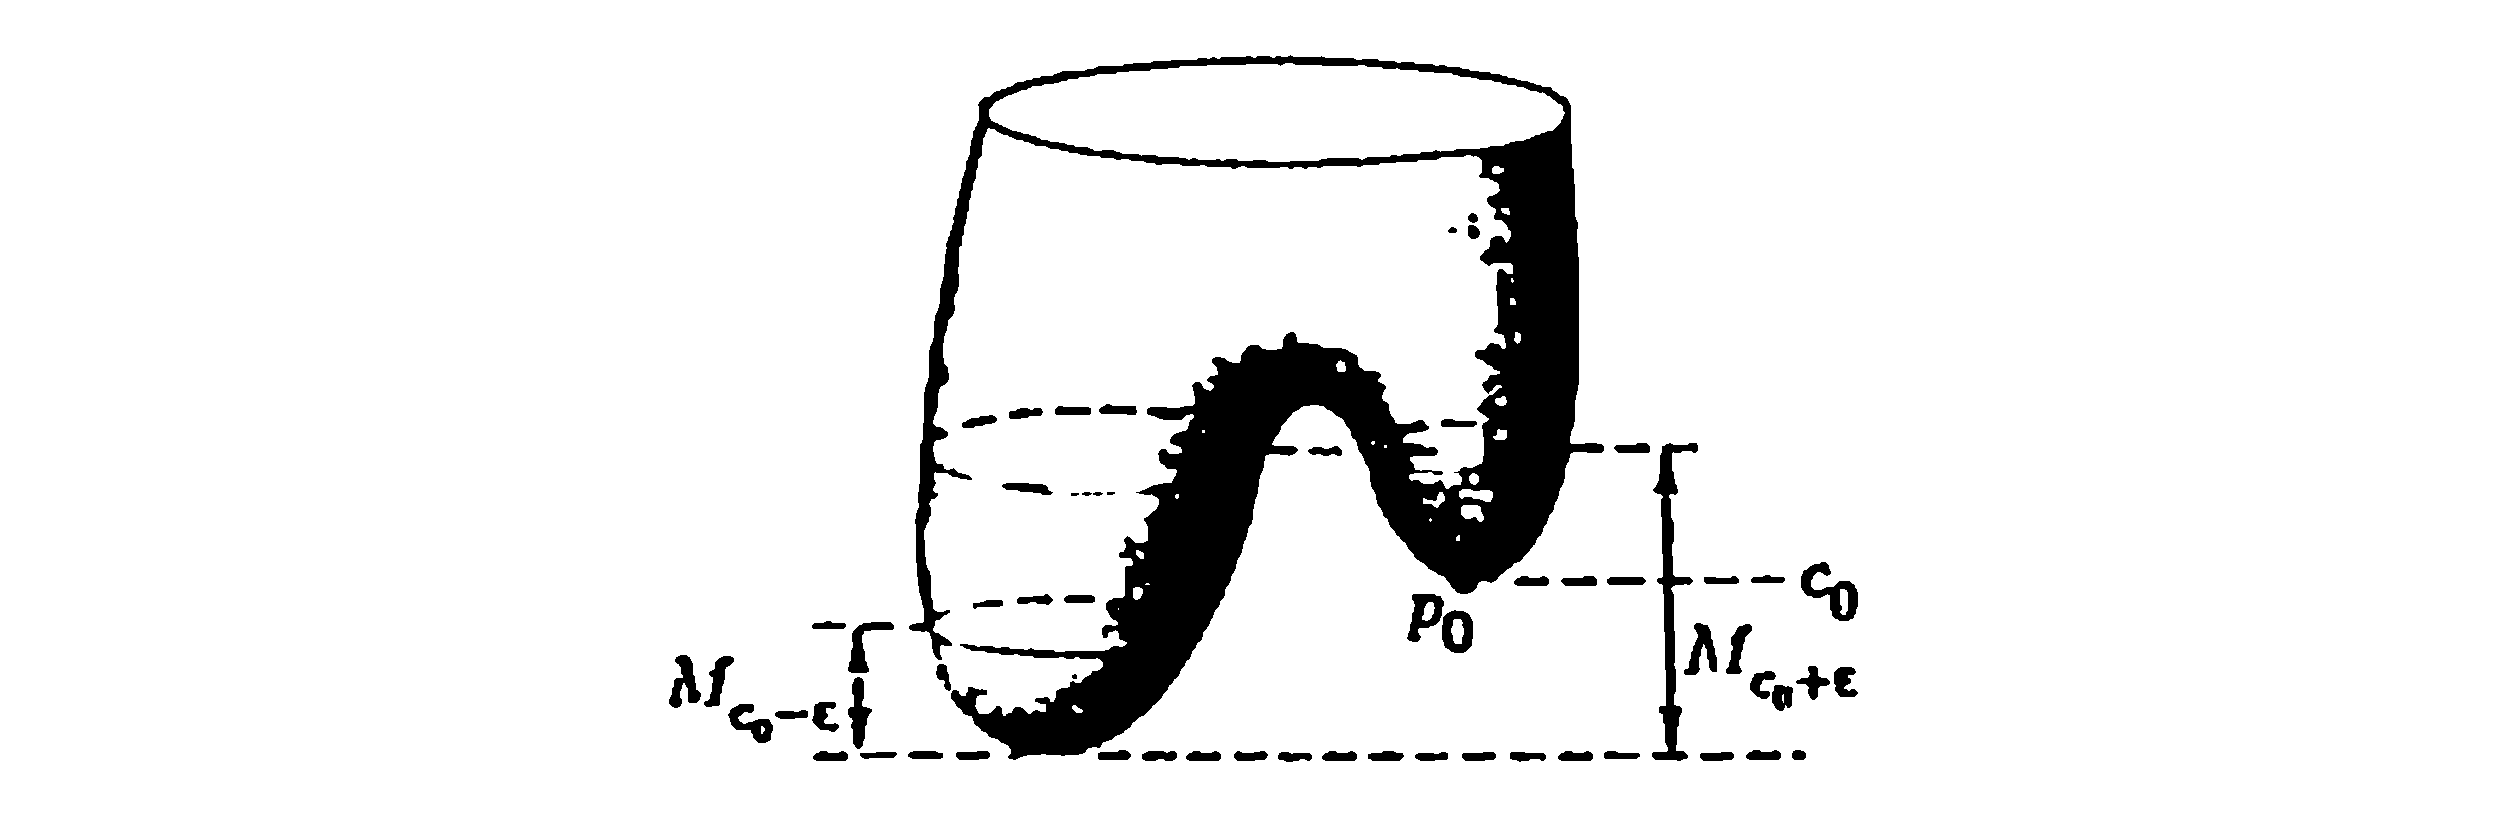
\includegraphics[width=\textwidth]{1-14.png}
\caption{Случай (а): индекс $p_0$ равен нулю.}
\label{fig:p0_index_zero}
\end{figure}

\indention{(б) Второй случай: индекс $p_0$ равен 1}

Запишем функцию $f$ в локальных координатах $(x, y)$ в стандартной форме (см. Теорему \ref{thm:morse_lemma_2d}):
\begin{equation}
f = -x^2 + y^2 + c_0,
\end{equation}
где мы поменяли местами $x$ и $y$ для соответствия обозначениям в общем случае, который будет рассмотрен в следующей главе. График функции $f$ в окрестности $p_0$ напоминает горный перевал (см. рисунок \ref{fig:p0_index_one}). Кривая, соответствующая $y = 0$, уходит вниз от $p_0$, а ортогональная ей кривая $x = 0$, наоборот, восходит из $p_0$ вверх. Таким образом, утверждение, что критическая точка имеет индекс $1$ эквивалентно тому, что нисходящее направление из критической точки одномерно.

\begin{figure}[ht]
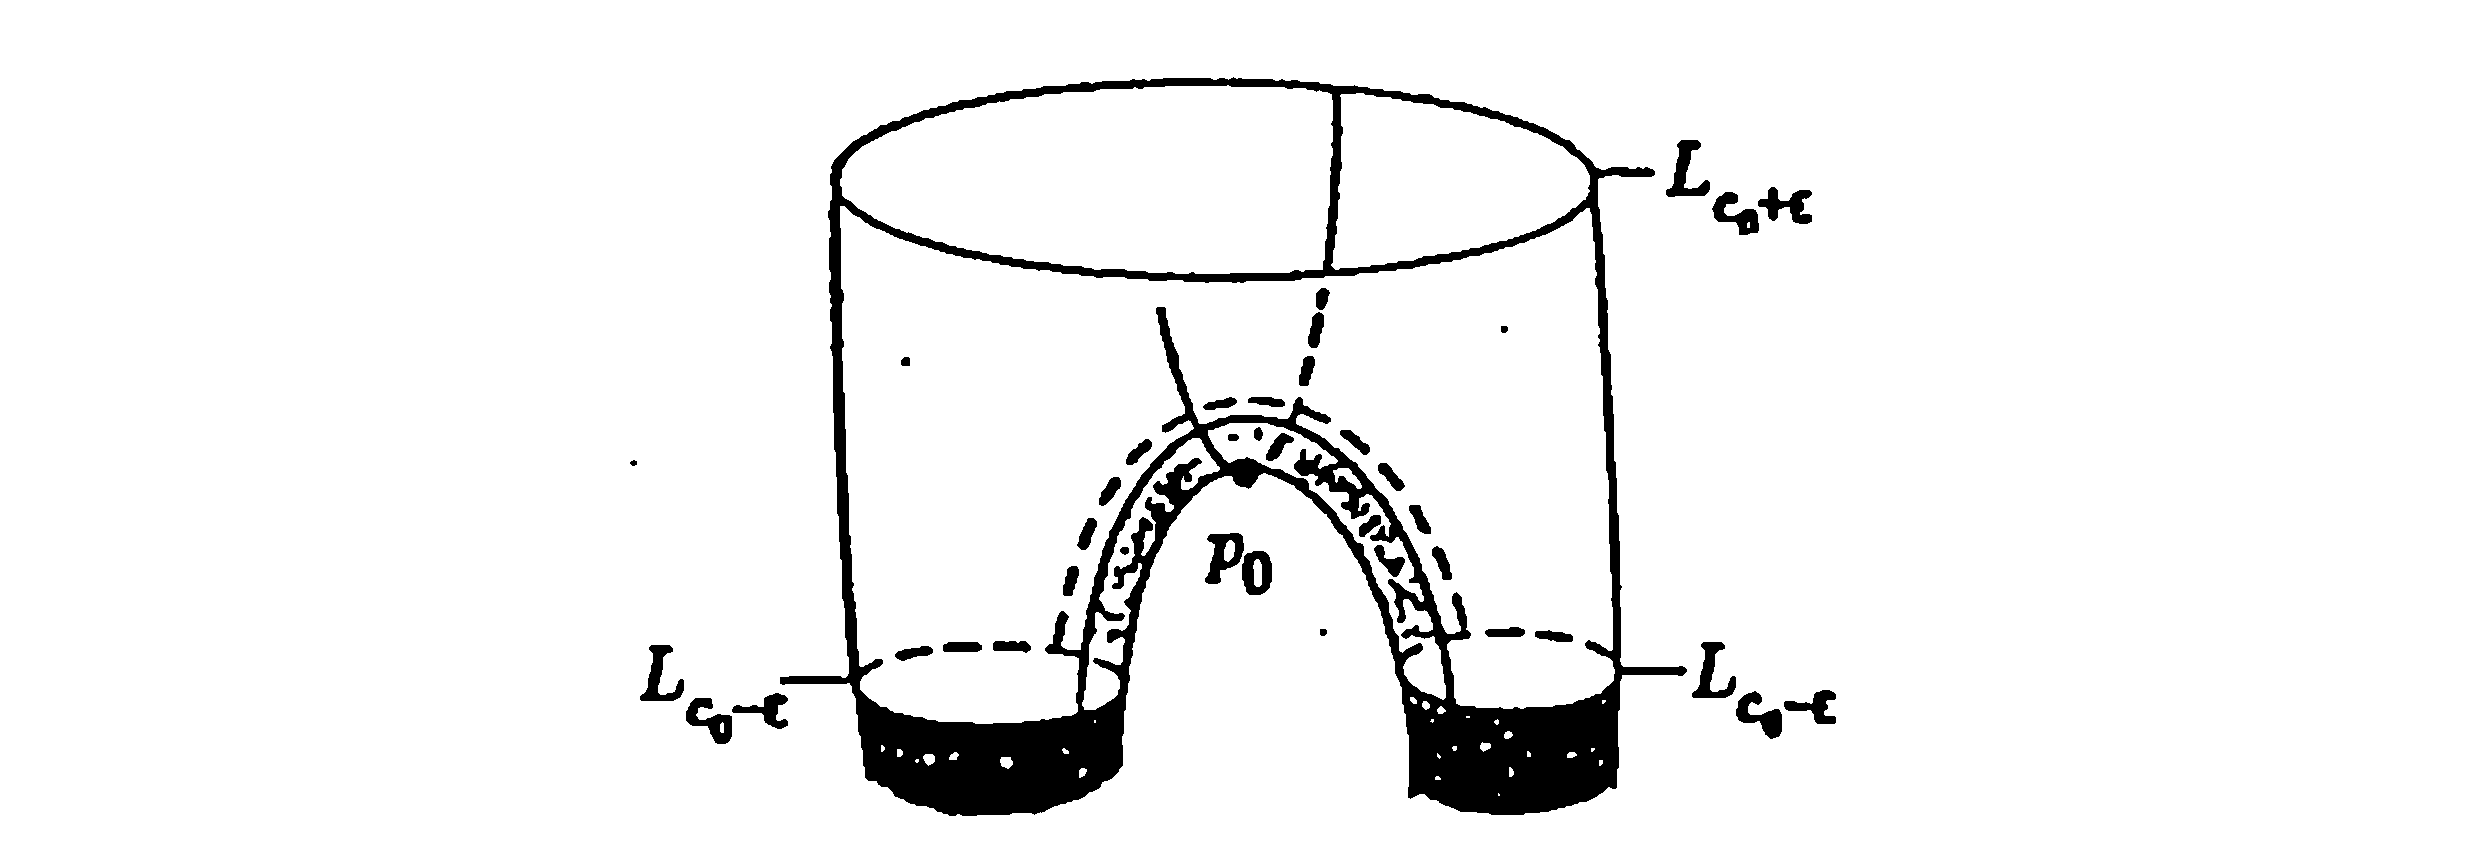
\includegraphics[width=\textwidth]{1-15.png}
\caption{График функции в окрестности критической точки индекса $1$.}
\label{fig:p0_index_one}
\end{figure}

Рассмотрим нисходящую кривую; добавив к ней точки, лежащие достаточно близко, получим узкую полосу, <<путь>>, проходящий по <<горному перевалу>> через $p_0$. Можно представлять эту полосу, как узкий мост, соединяющий разные участки границы $L_{c_0 - \epsilon}$ поверхности $M_{c_0 - \epsilon}$. На рисунке \ref{fig:p0_index_one_top_view} показан вид сверху графика с рисунка \ref{fig:p0_index_one}.

\begin{figure}[ht]
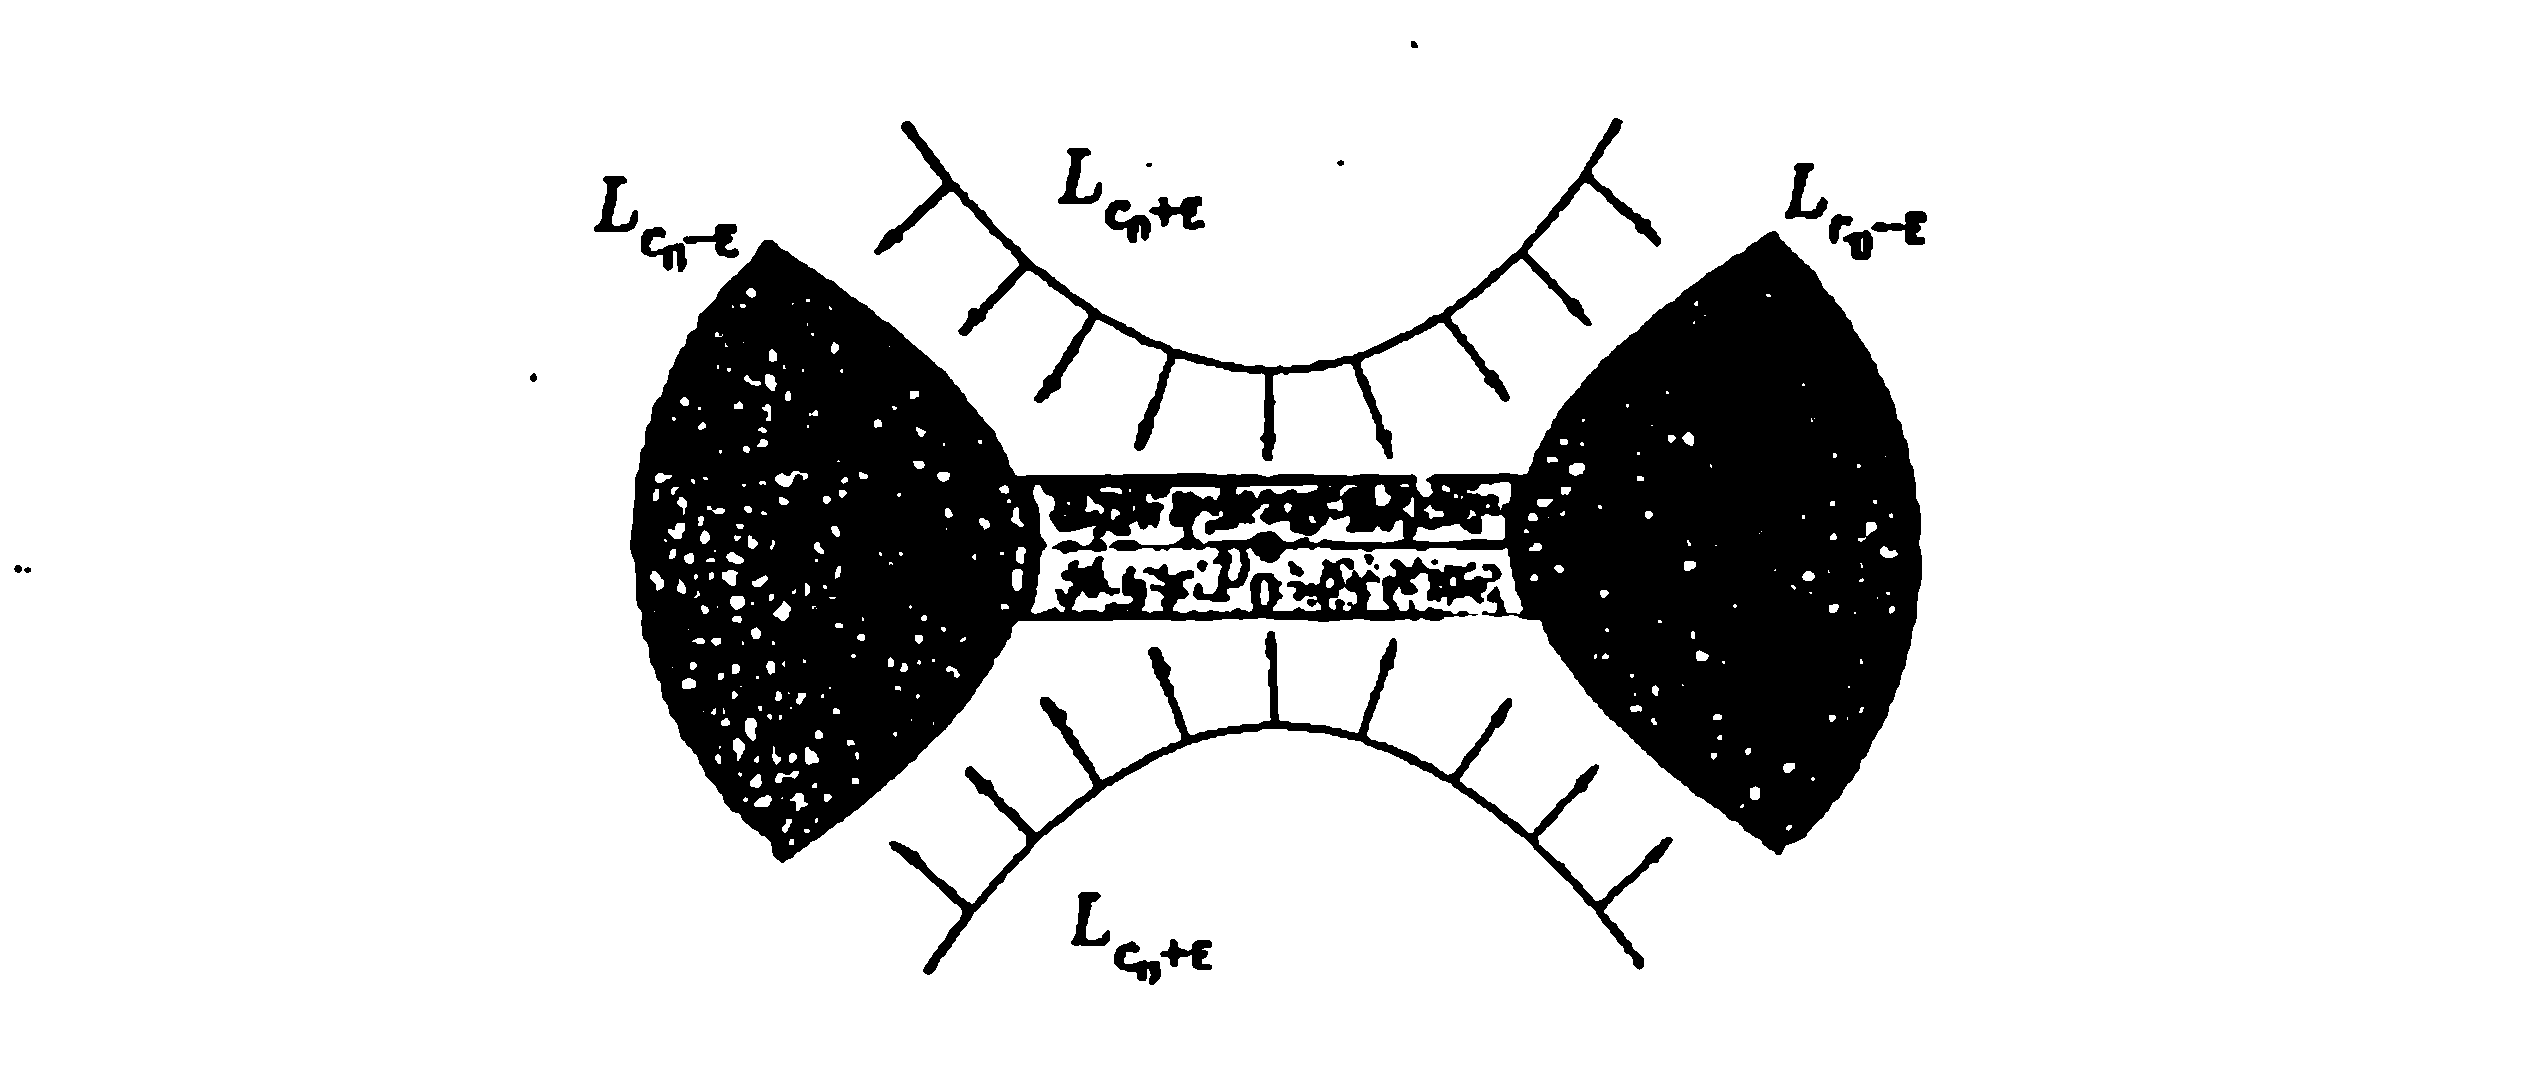
\includegraphics[width=\textwidth]{1-16.png}
\caption{Вид сверху графика с рисунка \ref{fig:p0_index_one}.}
\label{fig:p0_index_one_top_view}
\end{figure}

Закрашенная область на рисунке \ref{fig:p0_index_one_top_view} соответствует $M_{p_0 - \epsilon}$ и задаётся уравнением
\[
-x^2 + y^2 \leq - \epsilon,
\]
а затенённая область на рисунке \ref{fig:p0_index_one_top_view} соответствует мосту, соединяющему $M_{c_0 - \epsilon}$. Мост <<почти прямоугольный>> (диффеоморфен прямоугольнику), хоть и немного искривлён.

Отрезок $[0, 1]$ мы будем называть одномерным диском, или просто 1-диском, и будем обозначать как $D^1$. Концы отрезка $D^1$ являются его границей и обозначаются как $\d D^1$. Таким образом, $\d D^1$ состоит из двух точек.

Серый прямоугольный <<мостик>> на рисунке \ref{fig:p0_index_one_top_view} диффеоморфен произведению $D^1 \times D^1$, а его пересечение с $M_{c_0 - \epsilon}$ (показано жирными линиями на рисунке \ref{fig:p0_index_one_top_view}) соответствует паре противоположных рёбер $\d D^1 \times D^1$ (см. рисунок \ref{fig:handle_2d}).

\begin{figure}[ht]

\includegraphics[width=\textwidth]{1-17.png}
\caption{1-ручка $D^1 \times D^1$ и пара отрезков, которыми она приклеена к $M_{c_0 - \epsilon}$.}
\label{fig:handle_2d}
\end{figure}

Такой прямоугольник $D^1 \times D^1$ называется \emph{1-ручкой}, приклеенной к $M_{c_0 - \epsilon}$. Термин <<1-ручка>> иллюстрирует тот факт, что она соответствует критической точке индекса 1. Понимание этого термина лучше раскроется в дальнейшем, когда мы будем рассматривать трёхмерные ручки в третьей главе.

Поверхность $M_{c_0 + \epsilon}$ после того, как параметр $t$ прошёл критическое значение $c_0$, в локальных координатах описывается неравенством
\[
-x^2 + y^2 + c_0 \leq \epsilon.
\]

Сравним поверхности $M_{c_0 + \epsilon}$ и $M_{c_0 - \epsilon}$ с приклеенной 1-ручкой $D^1 \times D^1$ (рис. \ref{fig:p0_index_one_top_view}). Заметим, что мы можем стянуть $M_{c_0 + \epsilon}$ вдоль стрелок в поверхность $M_{c_0 - \epsilon} \cup D^1 \times D^1$. Следовательно,
\begin{equation}
M_{c_0 + \epsilon} \cong M_{c_0 - \epsilon} \cup D^1 \times D^1.
\label{eq:diff_1_handle}
\end{equation}

Таким образом, для критической точки $p_0$ индекса 1, изменение $M_t$ при прохождении параметра $t$ от $c_0 - \epsilon$ до $c_0 + \epsilon$ может быть описано как приклеивание 1-ручки к $M_{c_0 - \epsilon}$.

Строго говоря, поверхность $M_{c_0 - \epsilon} \cup D^1 \times D^1$ в правой части (\ref{eq:diff_1_handle}) в изображённом виде не является гладкой, поскольку граница $M_{c_0 - \epsilon} \cup D^1 \times D^1$ изгибается под прямым углом в четырёх углах, по которым приклеена 1-ручка $D^1 \times D^1$. Однако, это несложно исправить, используя известную технику <<сглаживания>> (см., например, TODO). Поэтому мы можем считать, что в диффеоморфизме (\ref{eq:diff_1_handle}) справа находится гладкая поверхность. В некоторых случаях мы будем использовать символ $\cong$ в (\ref{eq:diff_1_handle}) для обозначения гомеоморфизма, и в тех случаях, когда там нужно будет воспользоваться гладкостью поверхности, мы просто будем рассматривать поверхность $M_{c_0 + \epsilon}$. В любом случае, в дальнейших рассуждениях мы будем считать, что поверхность $M_{c_0 - \epsilon} \cup D^1 \times D^1$ гладкая.

\begin{figure}[ht]
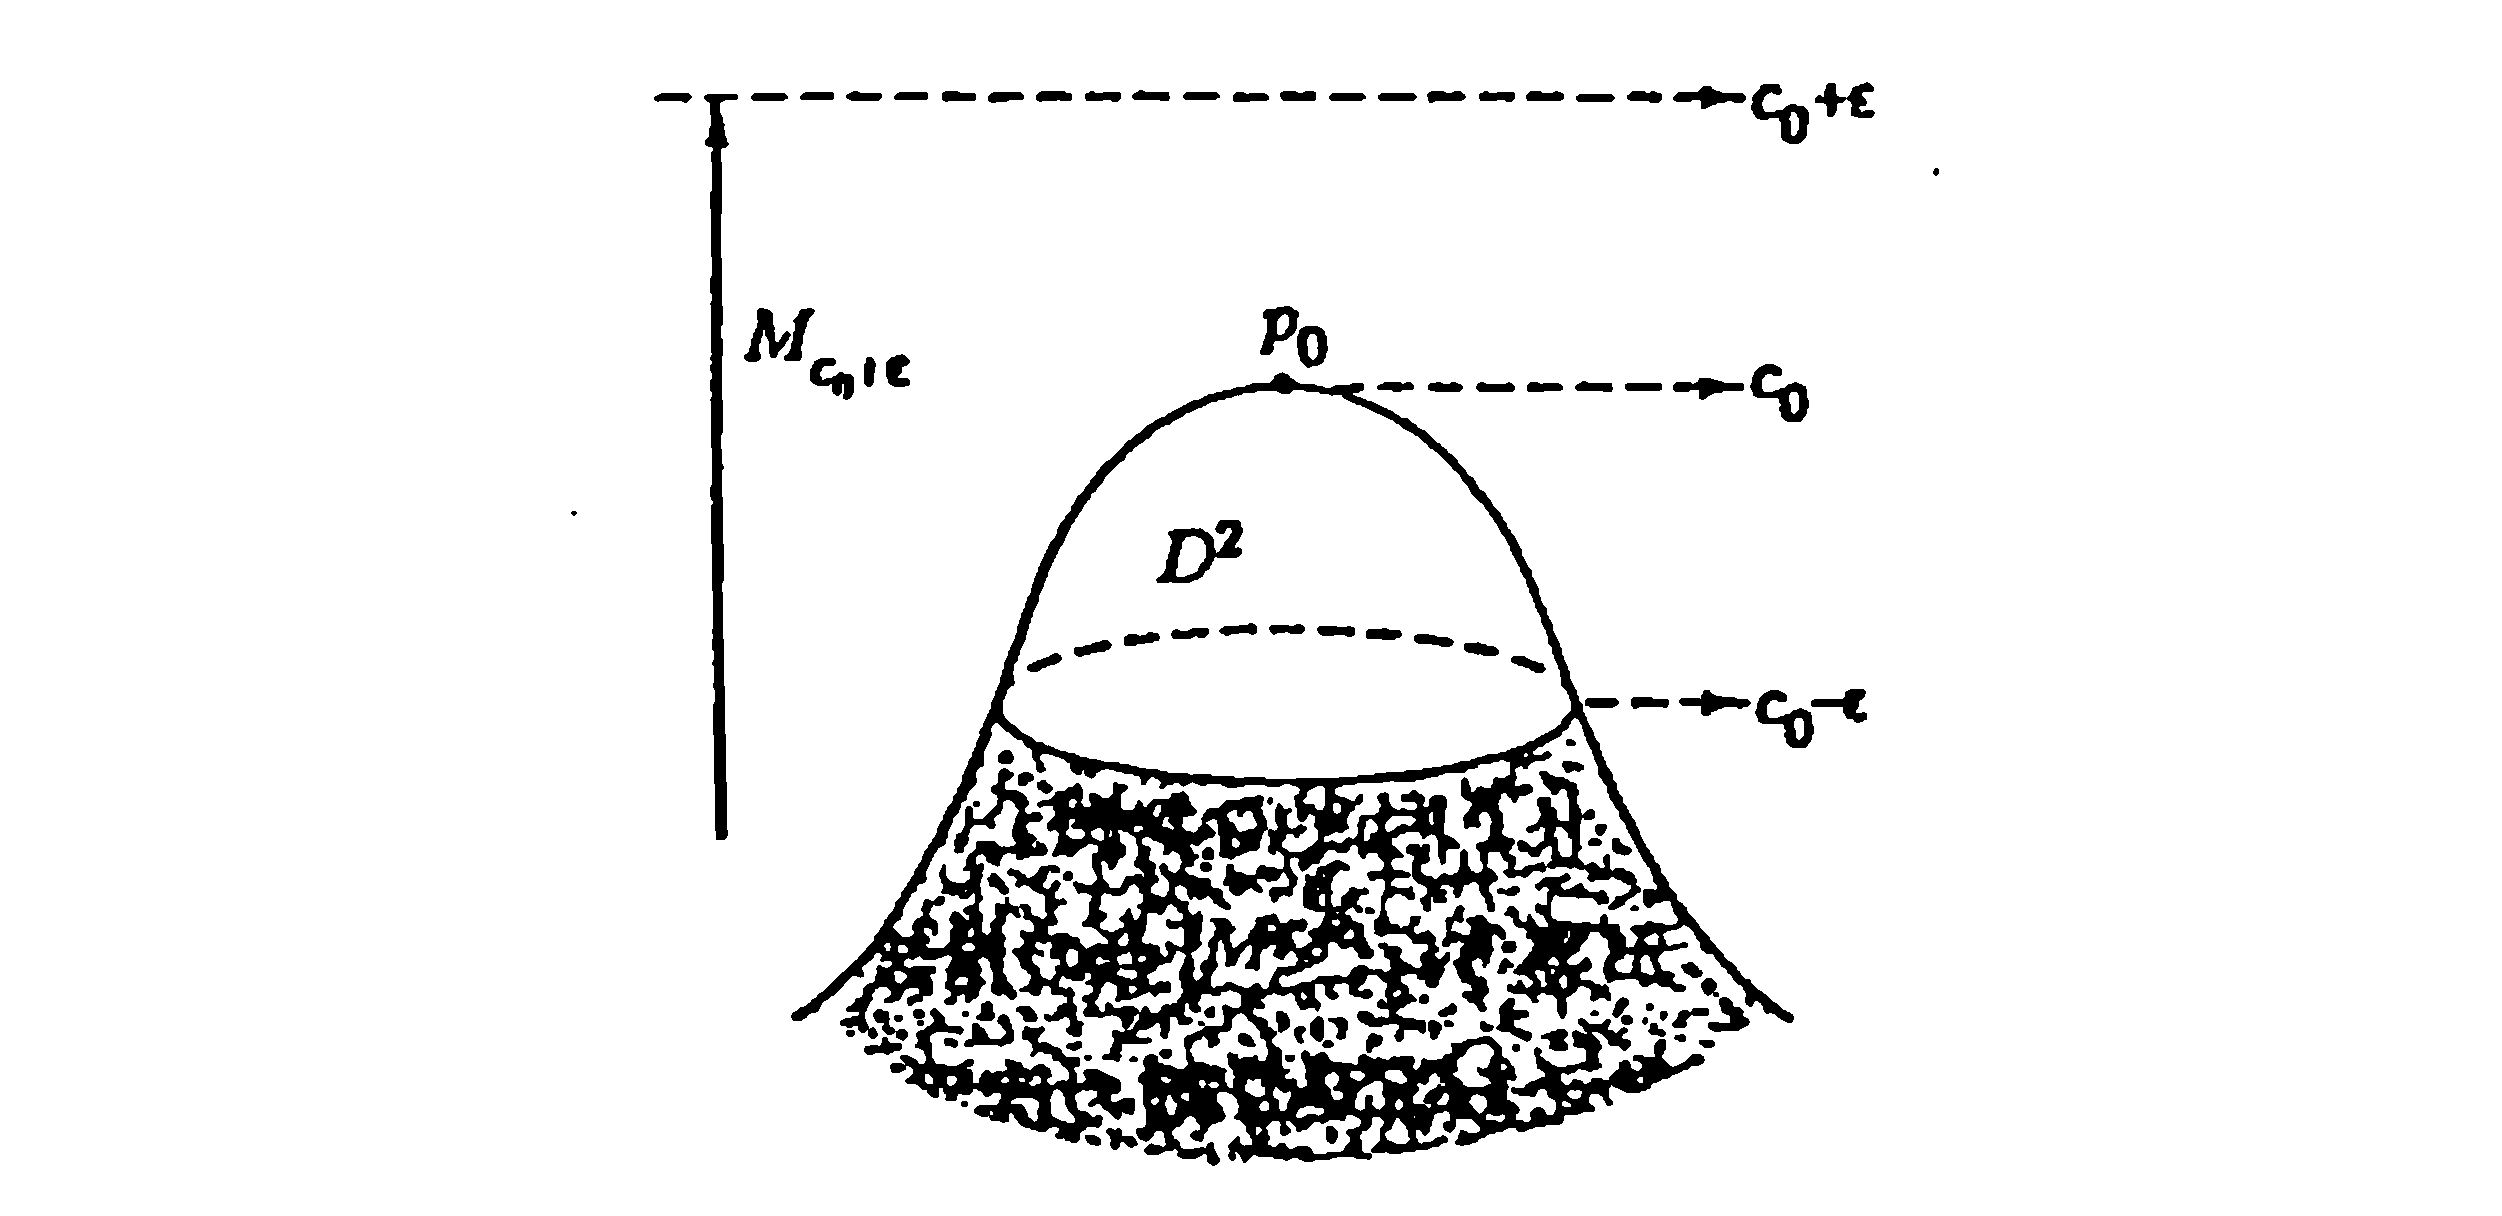
\includegraphics[width=\textwidth]{1-18.png}
\caption{Критическая точка индекса 2.}
\label{fig:p0_index_two}
\end{figure}

\indention{(в) Третий случай: индекс $p_0$ равен 2}

Запишем функцию $f$ в локальных координатах $(x, y)$ в стандартной форме (см. Теорему \ref{thm:morse_lemma_2d}):
\begin{equation}
f = -x^2 + -y^2 + c_0.
\end{equation}

В локальных координатах $(x, y)$ мы можем записать
\begin{equation}
M_{c_0 - \epsilon} = \{p \in M\,\mid\,f(p) \leq c_0 - \epsilon\} = \{(x, y)\,\mid\,x^2 + y^2 \geq \epsilon\},
\end{equation}

откуда $M_{c_0 - \epsilon}$ является дополнением к диску радиуса $\sqrt{\epsilon}$ (со включённой границей). На рисунке \ref{fig:p0_index_two} этот диск изображён как перевёрнутая чаша параболоида. Поверхность $M_{c_0 + \epsilon}$ получается приклейкой этой чаши к $M_{c_0 - \epsilon}$ по её границе:
\begin{equation}
M_{c_0 + \epsilon} \cong M_{c_0 - \epsilon} \cup D^2.
\label{eq:diff_2_handle}
\end{equation}

<<Шапочка>> $D^2$ называется \emph{2-ручкой}. Соотношение (\ref{eq:diff_1_handle}) означает, что при прохождении параметра $t$ от $c_0 - \epsilon$ к $c_0 + \epsilon$, поверхность $M_{c_0 + \epsilon}$ получается из $M_{c_0 - \epsilon}$ приклеиванием 2-ручки $D^2$. Заметим, что при приклеивании <<шапочки>> пропадает одна из граничных окружностей поверхности $M_{c_0 - \epsilon}$, таким образом, количество компонент связности границы уменьшается на 1.

\indention{(г) Разложение на ручки}

Вернёмся к функции Морса $f: M \to \R$.

По Лемме \ref{lm:finite_crit_pts_2d}, количество критических точек у функции $f$ конечно. Обозначим эти точки как
\[p_1, p_2, \ldots, p_n.\]

В следующей главе мы покажем, что можем <<пошевелить>> функцию Морса $f$ так, чтобы
\[f(p_i) \neq f(p_j) \text{ при } i \neq j.\]
Поэтому будем считать, что $f$ обладает этим свойством. Затем перенумеруем критические точки так, чтобы
\begin{equation}
f(p_1) < f(p_2) < \ldots < f(p_n).
\end{equation}
Обозначим $c_i = f(p_i)$. Тогда
\begin{equation}
c_1 < c_2 < \ldots < c_n.
\end{equation}
Очевидно, $c_1$ --- минимальное значение $f$, а $c_n$ --- максимальное значение.

Будем наблюдать, как изменяется поверхность $M_t$ при возрастании $t$, начиная с некоторого значения, меньшего $c_1$. При $t < c_1$, $M_t = \emptyset$. При прохождении значения $c_1$ появляется диск (чаша параболоида), и $M_t = D^2$. Так произойдёт, поскольку индекс $p_0$ равен нулю, т.~к. $c_1$ --- минимум $f$. Этот 2-диск соответствует критической точке индекса 0 и называется \emph{0-ручкой}. 2-ручка тоже является 2-диском, но 0-ручка соответствует чаше параболоида, а 2-ручка --- перевёрнутой чаше, или <<шапочке>>. (Возможна другая интерпретация индекса критической точки --- это количество нисходящих направлений. Поскольку 2-ручке-шапочке соответствует два направления спуска, то индекс критической точки равен 2. Для 1-ручки единственным нисходящим направлением будет центральная линия моста, см. Рисунок \ref{fig:p0_index_one_top_view}, поэтому индекс соответствующей критической точки равен 1. 0-ручка --- это чаша параболоида, у которой нет нисходящих направлений, поэтому индекс критической точки равен 0.)

Продолжая описанный процесс, каждый раз, когда $t$ проходит критическое значение $c_i$, мы приклеиваем 0-, 1- или 2-ручку к $M_{c_i - \epsilon}$ в зависимости от индекса соответствующей критической точки $p_i$ (<<приклеивание>> 0-ручки означает добавление ручки к $M_{c_i - \epsilon}$ в качестве новой связной компоненты).

Последнее значение $c_n$ является максимумом $f$, поэтому оно соответсвует 2-ручке. Границей поверхности $M_{c_0 - \epsilon}$ является окружность, по которой приклеивается эта 2-ручка, завершающая замкнутую поверхность $M$. Таким образом, мы показали справедливость следующей теоремы.

\begin{theorem} (Разложение на ручки замкнутой поверхности). Если на замкнутой поверхности $M$ задана функция Морса $f : M \to \R$, то $M$ может быть представлена как объединение конечного числа 0-, 1- и 2-ручек.
\end{theorem}

В следующей главе мы докажем существование функции Морса на любой замкнутой поверхности $M$, из чего следует, что любая замкнутая поверхность может быть разложена на ручки.

\indention{Краткое содержание главы}
\begin{itemize}
\item[1.1] Критические точки функции бывают вырожденными и невырожденными.
\item[1.2] Функция, у которой все критические точки невырождены, называется функцией Морса.
\item[1.3] Если функция Морса $f$ определена на замкнутой поверхности $M$, то мы можем исследовать $M$, рассматривая множества подуровня функции $f$.
\item[1.4] Каждый раз, когда значение $f$ проходит через критическое значение, к поверхности подуровня приклеивается ручка. Индекс ручки совпадает с индексом соответствующей критической точки.
\item[1.5] Таким образом, замкнутая поверхность $M$ может быть разложена в объединение конечного числа ручек.
\end{itemize}

\indention{Упражнения}
\begin{enumerate}
\item Замкнутая поверхность $M$ получена склейкой двух дисков $D^1$ и $D^2$ по диффеоморфизму $h: \d D^1 \to \d D^2$. Докажите, что $M \cong S^2$, используя Лемму \ref{lm:diff_extension_disk}.

\item Пусть окружность $S^1$ является границей диска $D^2$.

(а) Докажите, что любой гомеоморфизм $h: S^1 \to S^1$ можно продолжить до гомеоморфизма $H: D^2 \to D^2$.

(б) Докажите, что любой диффеоморфизм $h: S^1 \to S^1$ можно продолжить до диффеоморфизма $H: D^2 \to D^2$.

\item Тор $S^1 \times S^1$ параметризован углами $\theta$ и $\phi$, соответствующими точкам окружностей. Определим функцию
\[
f(\theta, \phi) = (R + r\cos \phi) \cos \theta,
\]
где $R > r$ --- положительные константы. Докажите, что $f$ --- функция Морса, и найдите её критические точки и их индексы.

\end{enumerate}


\end{document}